\section{Tổng quan bộ dữ liệu và phân tích khám phá dữ liệu}

\refstepcounter{subsection}
\subsection*{\thesubsection\quad Giới thiệu bộ dữ liệu Superstore Sales}

Bộ dữ liệu được sử dụng là Superstore Sales, phản ánh hoạt động bán hàng trong lĩnh vực bán lẻ. Dữ liệu bao gồm các thông tin liên quan đến đơn hàng, khách hàng, sản phẩm, khu vực bán hàng, doanh thu, số lượng bán, chiết khấu và lợi nhuận. Đây là những biến quan trọng để phân tích tình hình kinh doanh, đánh giá hiệu quả bán hàng và nhận diện xu hướng tiêu dùng của khách hàng. Việc lựa chọn bộ dữ liệu này phù hợp với mục tiêu nghiên cứu của đồ án, đó là phân tích doanh số bán hàng và xu hướng tiêu dùng của khách hàng trong lĩnh vực bán lẻ dựa trên dữ liệu thực tế.

Sau khi làm sạch, bộ dữ liệu gồm 10.194 dòng và 26 cột. Khoảng thời gian ghi nhận đơn hàng kéo dài từ ngày 03/01/2023 đến ngày 30/12/2026. Các nhóm biến chính trong bộ dữ liệu được trình bày trong Bảng \ref{tab:nhom-bien}.

\begin{table}[H]
\centering
\caption{Các nhóm biến chính trong bộ dữ liệu Superstore Sales}
\label{tab:nhom-bien}
\begin{tabular}{p{4cm} p{9cm}}
\hline
\textbf{Nhóm biến} & \textbf{Các trường dữ liệu tiêu biểu} \\
\hline
Thông tin đơn hàng & Order ID, Order Date, Ship Date, Ship Mode, Shipping Days \\
\hline
Thông tin khách hàng & Customer ID, Customer Name, Segment \\
\hline
Thông tin địa lý & Country/Region, City, State/Province, Postal Code, Region \\
\hline
Thông tin sản phẩm & Product ID, Category, Sub-Category, Product Name \\
\hline
Thông tin kinh doanh & Sales, Quantity, Discount, Profit \\
\hline
Thông tin thời gian mở rộng & Year, Month, Month Name, Quarter \\
\hline
\end{tabular}
\end{table}

\refstepcounter{subsection}
\subsection*{\thesubsection\quad Kiểm tra cấu trúc và chất lượng dữ liệu}

Theo lý thuyết về tiền xử lý dữ liệu, trước khi tiến hành phân tích và xây dựng mô hình, dữ liệu cần được kiểm tra về cấu trúc, kiểu dữ liệu, giá trị thiếu, dữ liệu trùng lặp và mức độ phù hợp của các biến [1, 3]. Đối với bộ dữ liệu Superstore Sales, các trường ngày tháng như \textit{Order Date} và \textit{Ship Date} được chuẩn hóa về kiểu dữ liệu thời gian; các biến định lượng như \textit{Sales}, \textit{Quantity}, \textit{Discount} và \textit{Profit} được sử dụng cho phân tích thống kê và trực quan hóa.

Kết quả kiểm tra cho thấy bộ dữ liệu sau làm sạch không còn giá trị thiếu và không có dòng dữ liệu trùng lặp. Điều này giúp bảo đảm dữ liệu đầu vào có tính đầy đủ và nhất quán cho các bước phân tích tiếp theo. Tóm tắt chất lượng dữ liệu được trình bày trong Bảng \ref{tab:chat-luong-du-lieu}.

\begin{table}[H]
\centering
\caption{Tổng quan chất lượng dữ liệu sau làm sạch}
\label{tab:chat-luong-du-lieu}
\begin{tabular}{|l|r|}
\hline
\textbf{Chỉ tiêu} & \textbf{Giá trị} \\
\hline
Số dòng dữ liệu & 10.194 \\
\hline
Số cột dữ liệu & 26 \\
\hline
Số giá trị thiếu & 0 \\
\hline
Số dòng trùng lặp & 0 \\
\hline
Số đơn hàng khác nhau & 5.111 \\
\hline
Số khách hàng khác nhau & 804 \\
\hline
Số sản phẩm khác nhau & 1.862 \\
\hline
\end{tabular}
\end{table}

\begin{figure}[H]
\centering
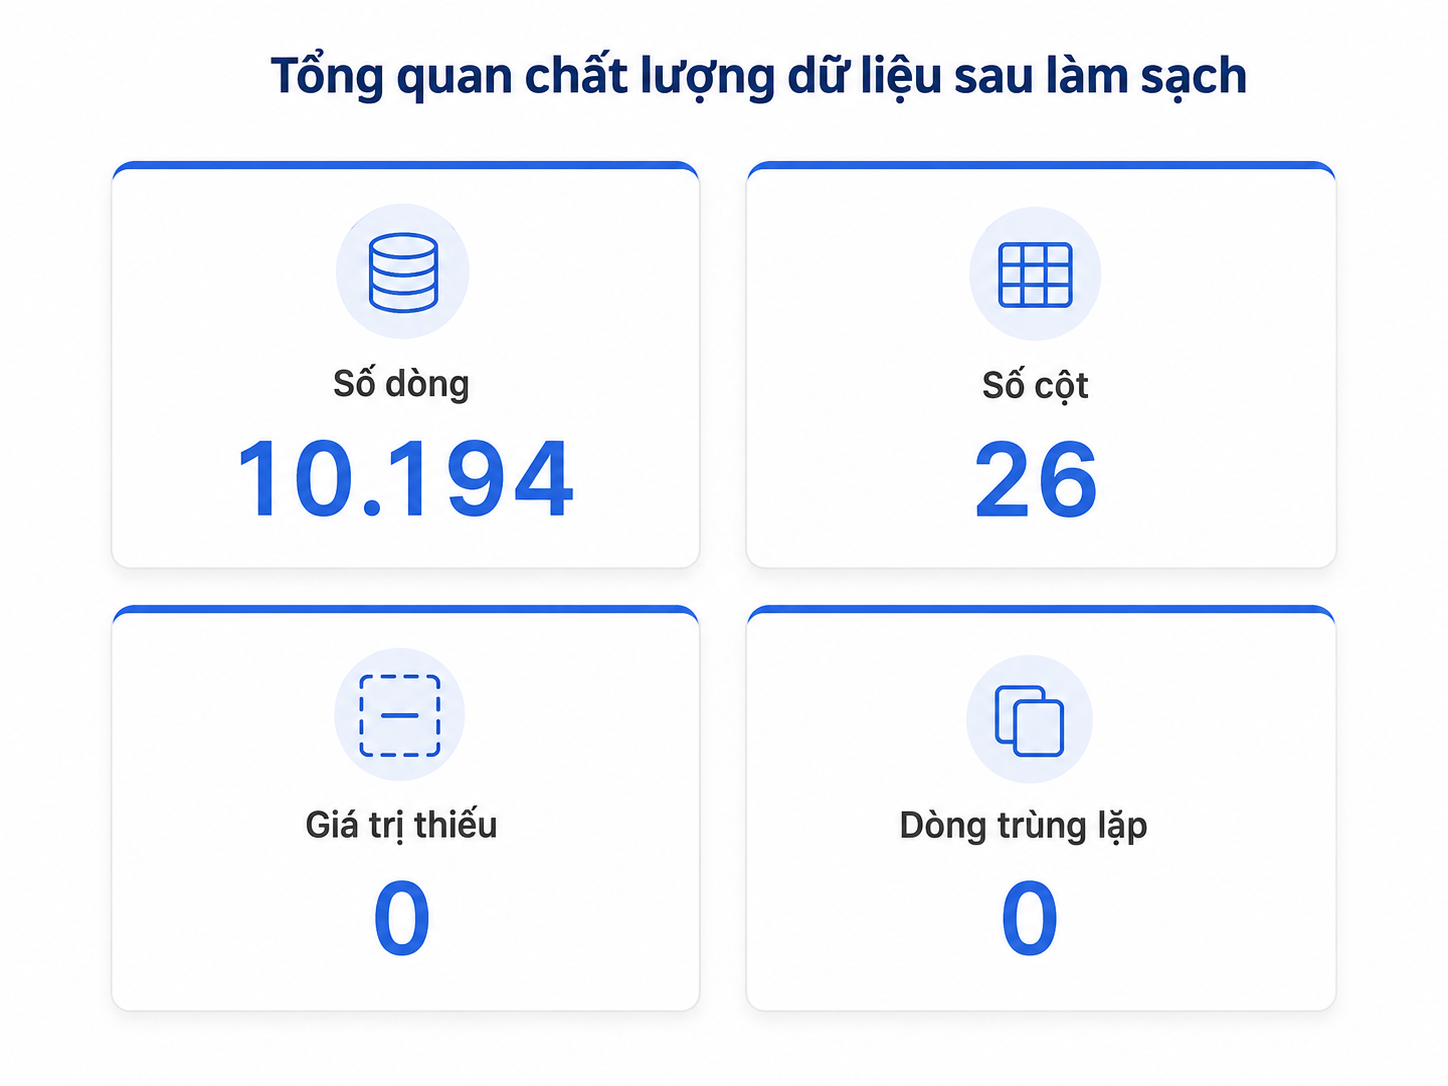
\includegraphics[width=0.85\textwidth]{images/anh_chuong3/hinh_3_8_tong_quan_chat_luong_du_lieu.png}
\caption{Tổng quan chất lượng dữ liệu sau làm sạch}
\label{fig:chat-luong-du-lieu}
\end{figure}

\refstepcounter{subsection}
\subsection*{\thesubsection\quad Thống kê mô tả các biến định lượng}

Thống kê mô tả là bước quan trọng trong phân tích khám phá dữ liệu, giúp tóm tắt đặc điểm phân bố của các biến và nhận diện những điểm đáng chú ý trong dữ liệu [1, 2]. Trong đồ án này, các biến định lượng chính gồm doanh thu, số lượng bán, chiết khấu và lợi nhuận. Bảng \ref{tab:thong-ke-mo-ta} trình bày thống kê mô tả của các biến này.

\begin{table}[H]
\centering
\caption{Thống kê mô tả các biến định lượng chính}
\label{tab:thong-ke-mo-ta}
\begin{tabular}{|l|r|r|r|r|}
\hline
\textbf{Biến} & \textbf{Trung bình} & \textbf{Trung vị} & \textbf{Nhỏ nhất} & \textbf{Lớn nhất} \\
\hline
Sales & 228,23 & 53,91 & 0,44 & 22.638,48 \\
\hline
Quantity & 3,79 & 3,00 & 1,00 & 14,00 \\
\hline
Discount & 0,16 & 0,20 & 0,00 & 0,80 \\
\hline
Profit & 28,67 & 8,69 & -6.599,98 & 8.399,98 \\
\hline
\end{tabular}
\end{table}

Kết quả thống kê cho thấy doanh thu trung bình của một dòng giao dịch là 228,23, trong khi trung vị chỉ đạt 53,91. Sự chênh lệch này cho thấy phân bố doanh thu có xu hướng lệch phải, tức là phần lớn giao dịch có giá trị nhỏ hoặc trung bình, trong khi một số giao dịch có giá trị rất lớn làm tăng giá trị trung bình. Lợi nhuận cũng có biên độ dao động lớn, từ -6.599,98 đến 8.399,98, phản ánh sự khác biệt đáng kể về hiệu quả kinh doanh giữa các giao dịch.

\refstepcounter{subsection}
\subsection*{\thesubsection\quad Phân tích tổng quan doanh thu, lợi nhuận và số lượng bán}

Tổng doanh thu của bộ dữ liệu đạt 2.326.534,35; tổng lợi nhuận đạt 292.296,81; tổng số lượng sản phẩm bán ra là 38.654. Ngoài ra, dữ liệu ghi nhận 1.901 dòng giao dịch có lợi nhuận âm với tổng mức lỗ là -157.038,93. Điều này cho thấy mặc dù hoạt động kinh doanh tổng thể có lãi, vẫn tồn tại một nhóm giao dịch gây lỗ cần được phân tích sâu hơn, đặc biệt khi xem xét theo danh mục sản phẩm, khu vực và mức chiết khấu.

\begin{table}[H]
\centering
\caption{Một số chỉ tiêu tổng quan về hoạt động kinh doanh}
\label{tab:kpi-tong-quan}
\begin{tabular}{|l|r|}
\hline
\textbf{Chỉ tiêu} & \textbf{Giá trị} \\
\hline
Tổng doanh thu & 2.326.534,35 \\
\hline
Tổng lợi nhuận & 292.296,81 \\
\hline
Tổng số lượng bán & 38.654 \\
\hline
Số đơn hàng & 5.111 \\
\hline
Số khách hàng & 804 \\
\hline
Số dòng có lợi nhuận âm & 1.901 \\
\hline
Tổng lỗ từ các dòng lợi nhuận âm & -157.038,93 \\
\hline
\end{tabular}
\end{table}

\refstepcounter{subsection}
\subsection*{\thesubsection\quad Phân tích doanh thu và lợi nhuận theo thời gian}

Phân tích theo thời gian giúp nhận diện xu hướng biến động của doanh số và lợi nhuận trong từng giai đoạn. Đây là nội dung trực tiếp trả lời câu hỏi nghiên cứu: doanh số bán hàng thay đổi như thế nào theo thời gian. Kết quả tổng hợp theo năm được trình bày trong Bảng \ref{tab:theo-nam}.

\begin{table}[H]
\centering
\caption{Doanh thu, lợi nhuận và số lượng bán theo năm}
\label{tab:theo-nam}
\begin{tabular}{|r|r|r|r|r|}
\hline
\textbf{Năm} & \textbf{Doanh thu} & \textbf{Lợi nhuận} & \textbf{Số lượng bán} & \textbf{Số đơn hàng} \\
\hline
2023 & 494.040,21 & 51.684,30 & 7.813 & 995 \\
\hline
2024 & 472.993,03 & 62.020,97 & 8.086 & 1.053 \\
\hline
2025 & 613.933,58 & 82.665,20 & 10.018 & 1.340 \\
\hline
2026 & 745.567,53 & 95.926,35 & 12.737 & 1.723 \\
\hline
\end{tabular}
\end{table}

Từ Bảng \ref{tab:theo-nam}, có thể thấy doanh thu và lợi nhuận nhìn chung có xu hướng tăng qua các năm. Năm 2026 là năm có doanh thu cao nhất với 745.567,53 và lợi nhuận cao nhất với 95.926,35. Số đơn hàng và số lượng bán cũng tăng mạnh trong năm 2026, cho thấy quy mô hoạt động kinh doanh được mở rộng so với các năm trước.

\begin{figure}[H]
\centering
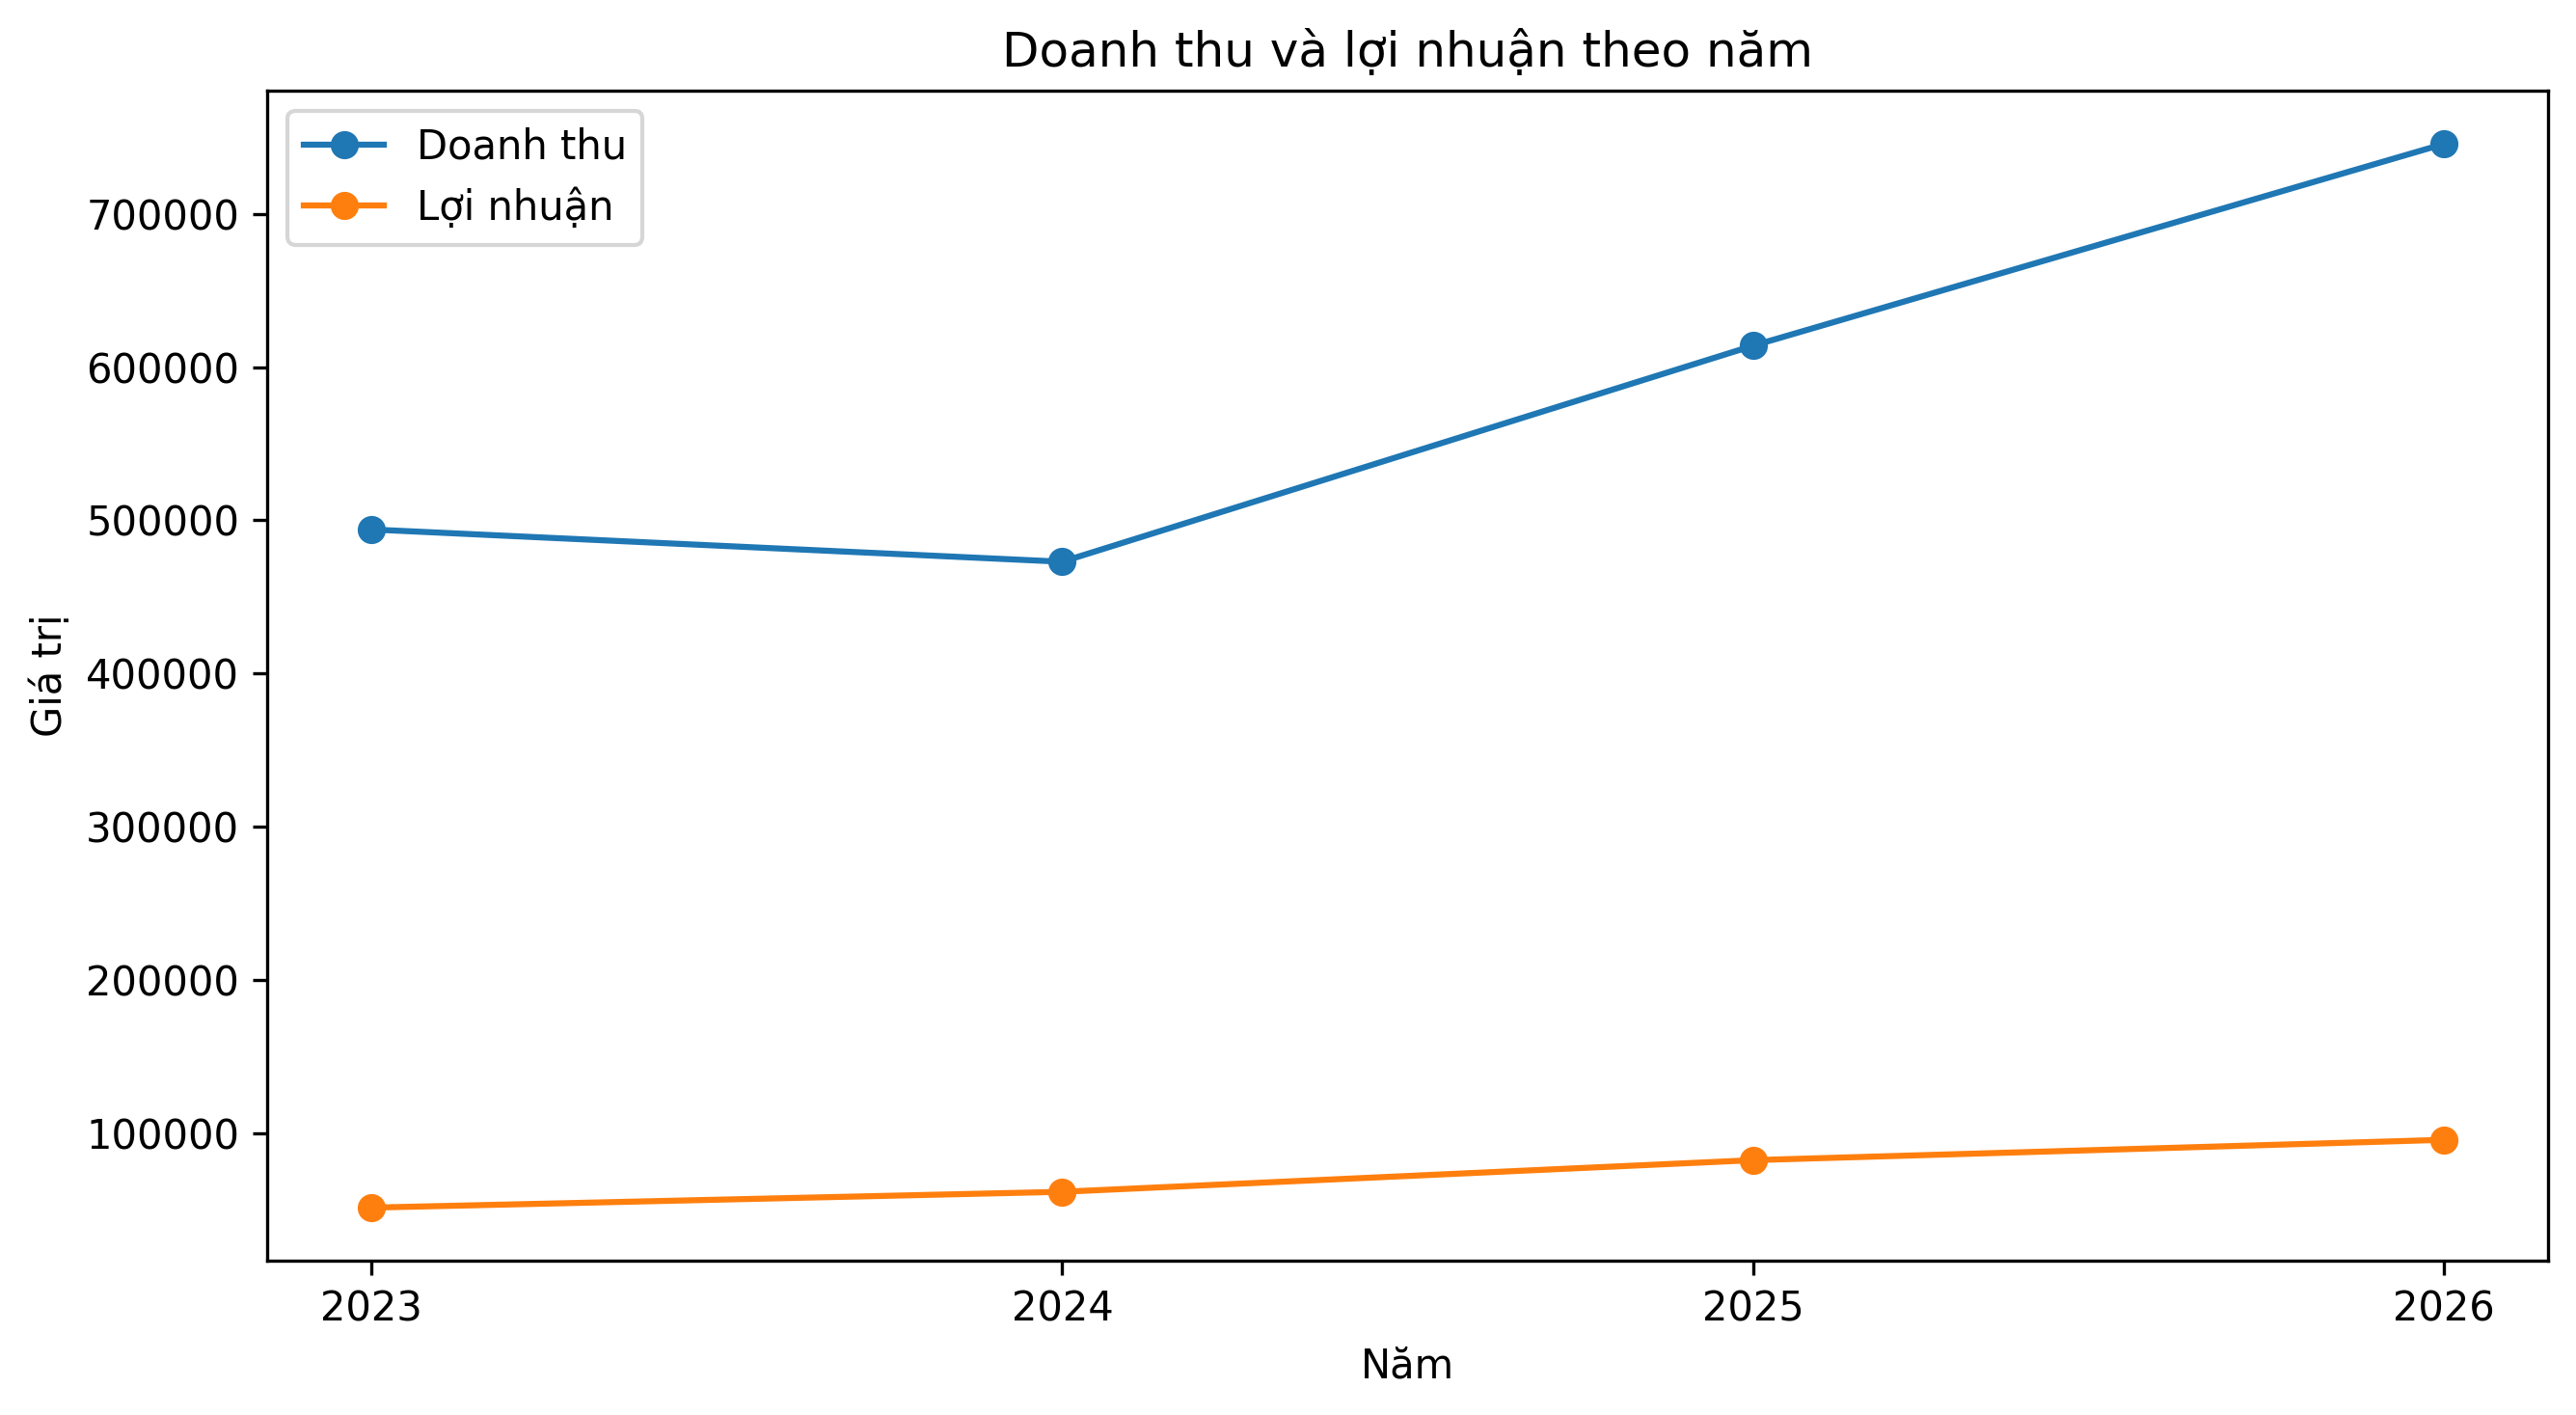
\includegraphics[width=0.9\textwidth]{images/anh_chuong3/hinh_3_1_doanh_thu_loi_nhuan_theo_nam.png}
\caption{Doanh thu và lợi nhuận theo năm}
\label{fig:doanh-thu-loi-nhuan-nam}
\end{figure}

Bên cạnh xu hướng theo năm, việc quan sát doanh thu theo tháng giúp nhận diện rõ hơn mức độ dao động trong từng giai đoạn. Hình \ref{fig:xu-huong-thang} thể hiện xu hướng doanh thu theo tháng trong toàn bộ giai đoạn nghiên cứu.

\begin{figure}[H]
\centering
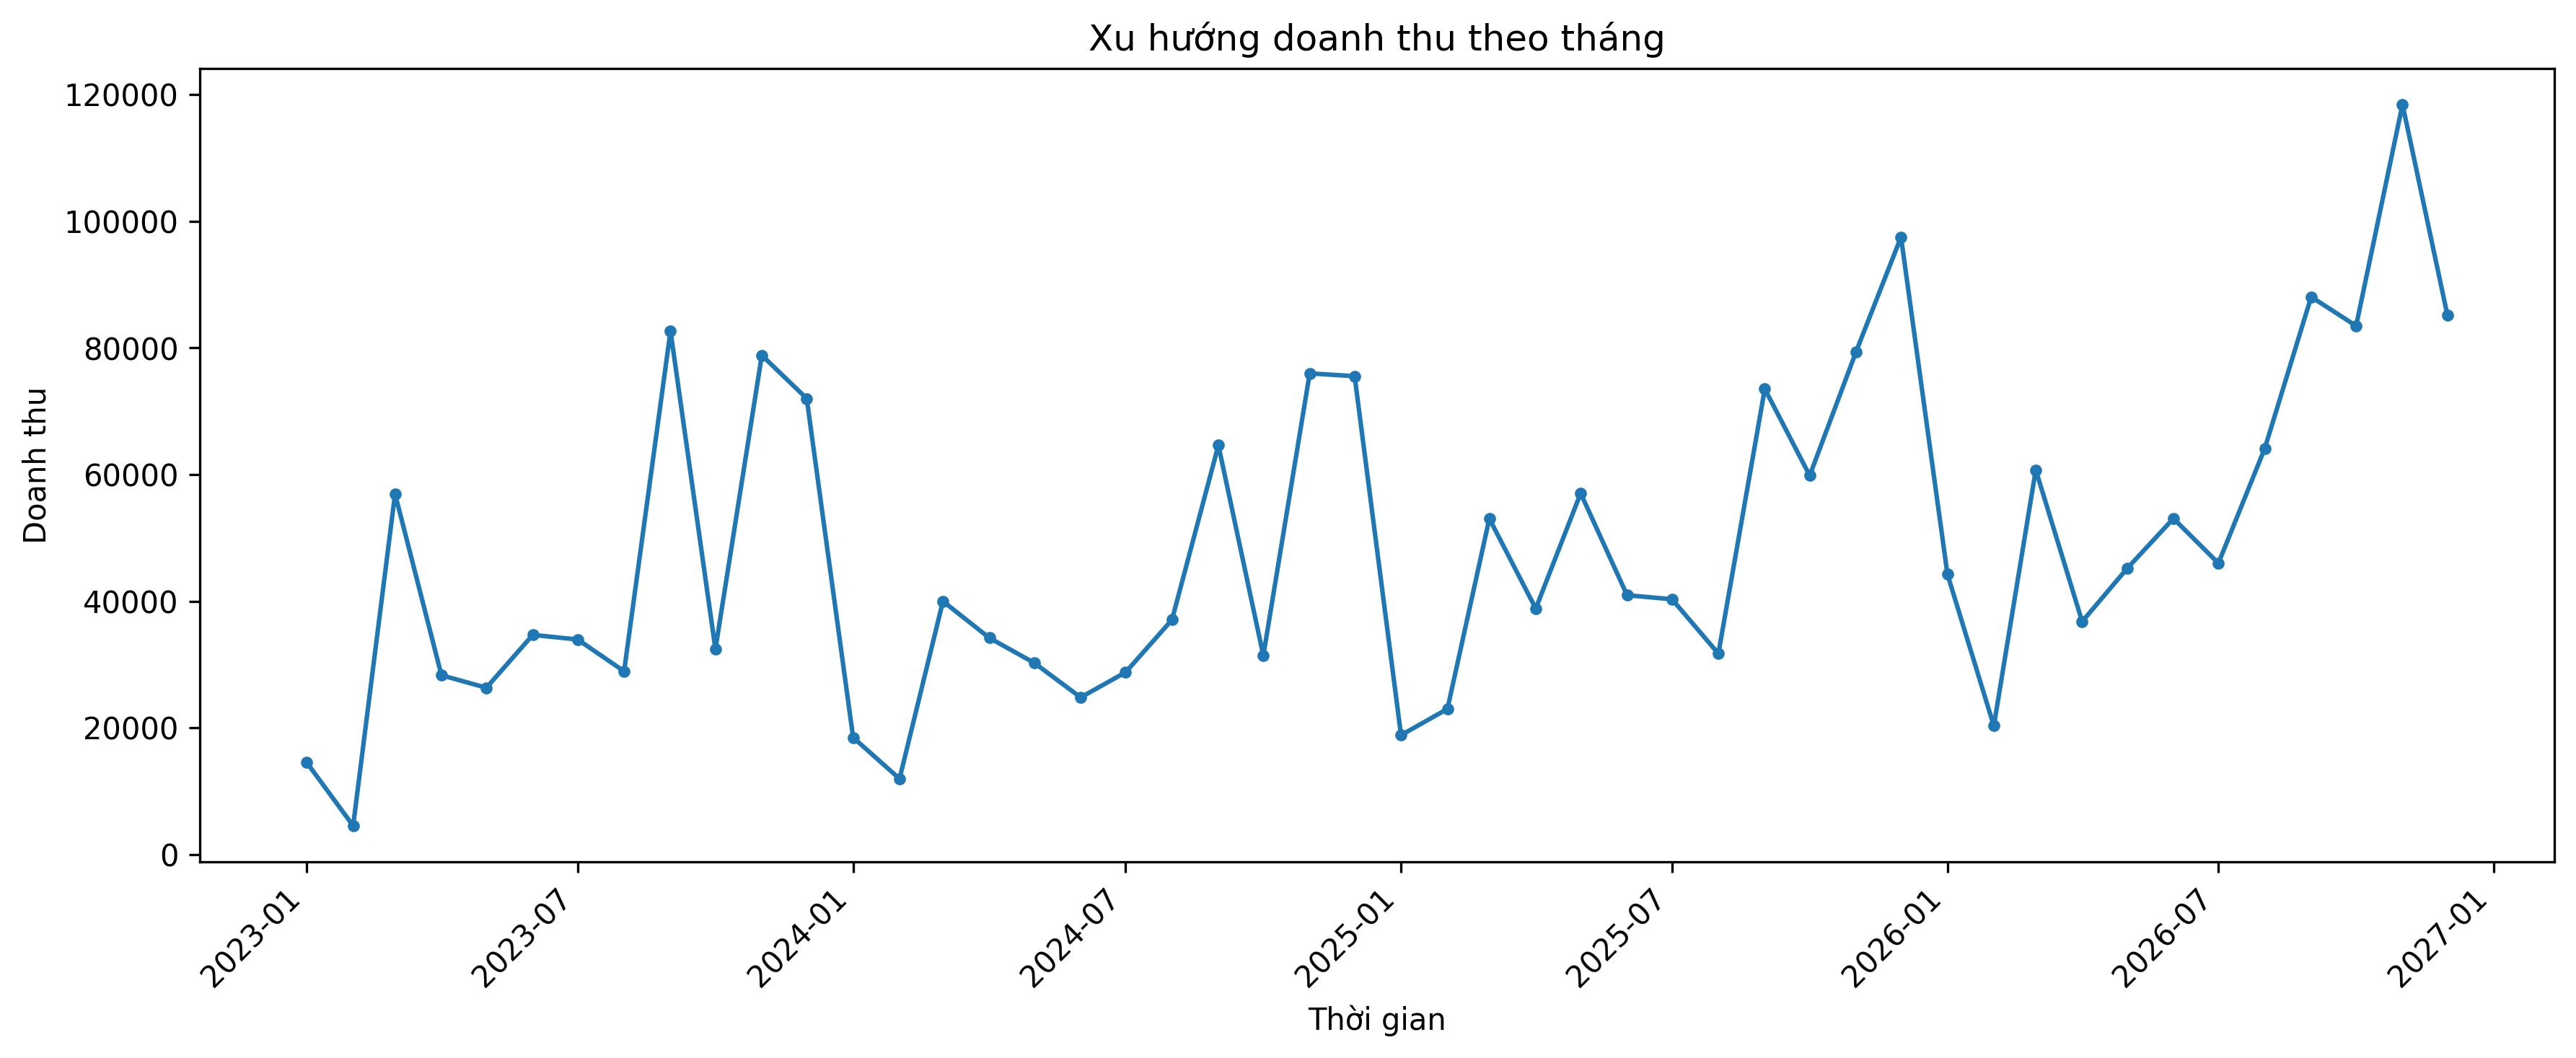
\includegraphics[width=0.95\textwidth]{images/anh_chuong3/hinh_3_7_xu_huong_doanh_thu_theo_thang.png}
\caption{Xu hướng doanh thu theo tháng}
\label{fig:xu-huong-thang}
\end{figure}

\refstepcounter{subsection}
\subsection*{\thesubsection\quad Phân tích theo khu vực bán hàng}

Phân tích theo khu vực giúp đánh giá mức độ đóng góp của từng vùng vào kết quả kinh doanh. Kết quả cho thấy khu vực West đạt doanh thu và lợi nhuận cao nhất, tiếp theo là East. Trong khi đó, South có doanh thu thấp nhất nhưng lợi nhuận vẫn cao hơn Central. Điều này cho thấy hiệu quả kinh doanh không chỉ phụ thuộc vào quy mô doanh thu mà còn chịu ảnh hưởng bởi cơ cấu sản phẩm, chiết khấu và khả năng sinh lợi của từng khu vực.

\begin{table}[H]
\centering
\caption{Doanh thu và lợi nhuận theo khu vực}
\label{tab:khu-vuc}
\begin{tabular}{|l|r|r|r|}
\hline
\textbf{Khu vực} & \textbf{Doanh thu} & \textbf{Lợi nhuận} & \textbf{Số đơn hàng} \\
\hline
West & 739.813,61 & 110.798,82 & 1.635 \\
\hline
East & 691.828,17 & 94.883,26 & 1.475 \\
\hline
Central & 503.170,67 & 39.865,31 & 1.179 \\
\hline
South & 391.721,91 & 46.749,43 & 822 \\
\hline
\end{tabular}
\end{table}

\begin{figure}[H]
\centering
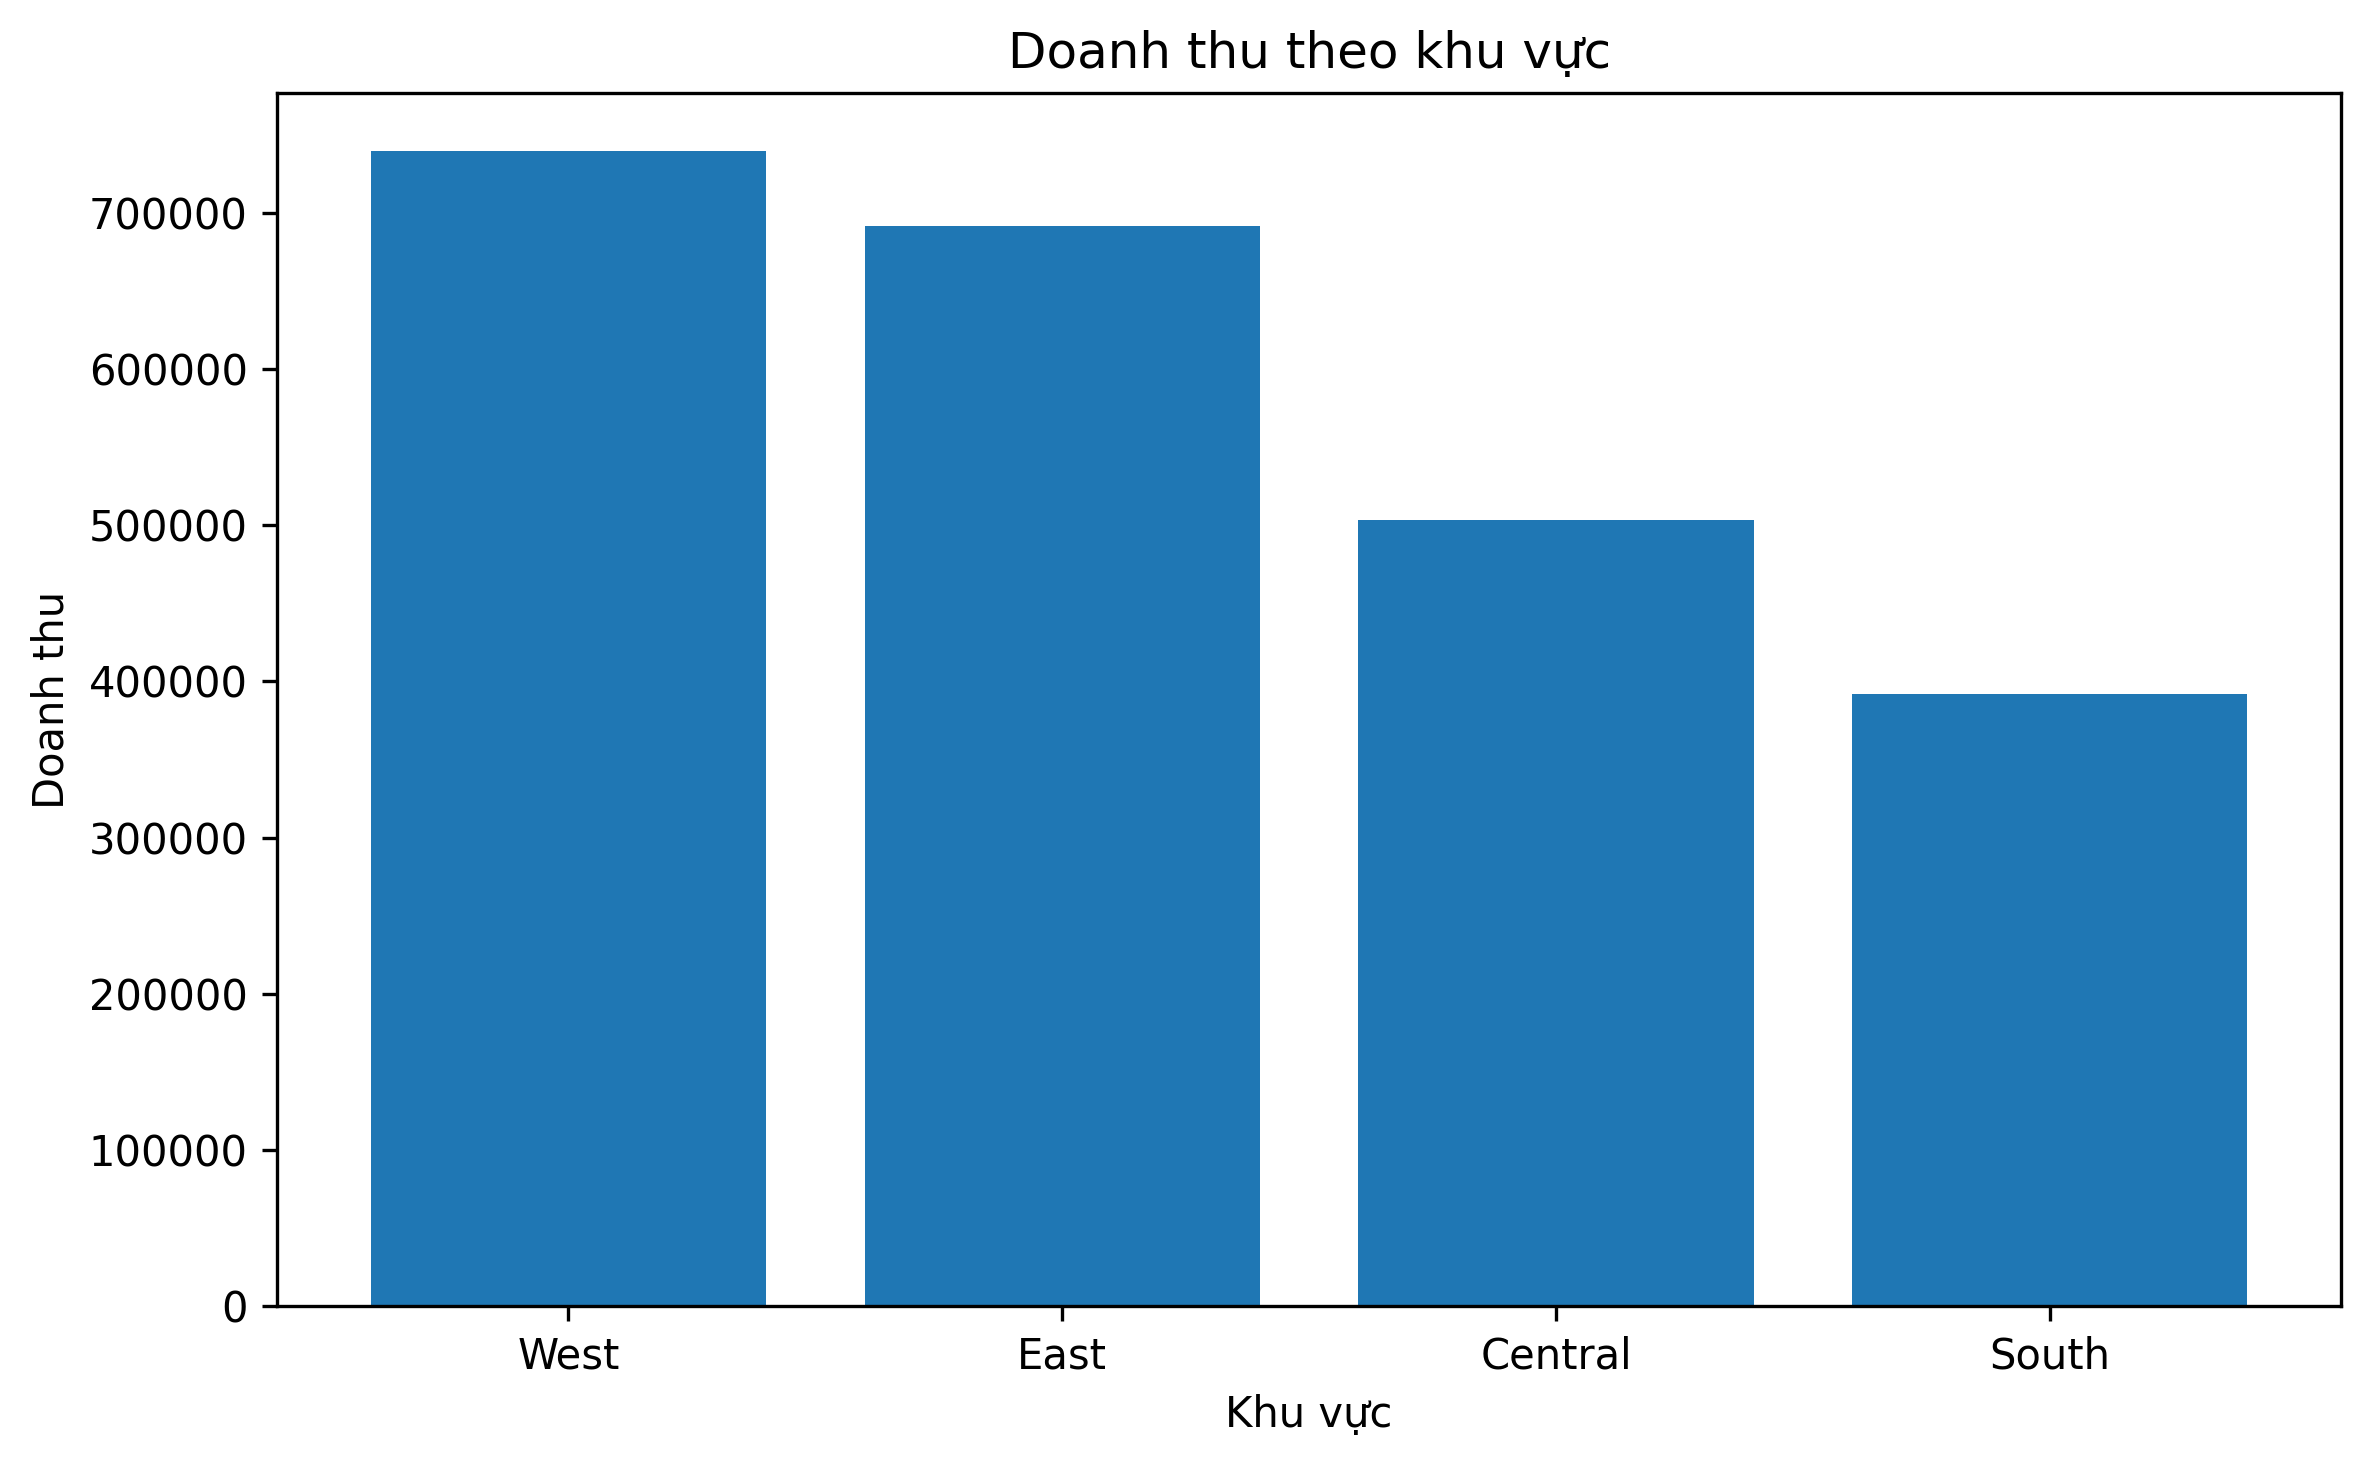
\includegraphics[width=0.85\textwidth]{images/anh_chuong3/hinh_3_2_doanh_thu_theo_khu_vuc.png}
\caption{Doanh thu theo khu vực}
\label{fig:doanh-thu-khu-vuc}
\end{figure}

\refstepcounter{subsection}
\subsection*{\thesubsection\quad Phân tích theo danh mục và tiểu danh mục sản phẩm}

Phân tích theo danh mục sản phẩm giúp xác định nhóm sản phẩm đóng góp chính vào doanh thu và lợi nhuận. Kết quả cho thấy Technology là danh mục có doanh thu và lợi nhuận cao nhất, với lợi nhuận đạt 146.543,38. Office Supplies có lợi nhuận cao thứ hai, trong khi Furniture tuy có doanh thu lớn nhưng lợi nhuận chỉ đạt 19.730,00. Điều này cho thấy Furniture có hiệu quả sinh lời thấp hơn so với hai danh mục còn lại.

\begin{table}[H]
\centering
\caption{Doanh thu, lợi nhuận và số lượng bán theo danh mục sản phẩm}
\label{tab:danh-muc}
\begin{tabular}{|l|r|r|r|}
\hline
\textbf{Danh mục} & \textbf{Doanh thu} & \textbf{Lợi nhuận} & \textbf{Số lượng bán} \\
\hline
Technology & 839.893,28 & 146.543,38 & 7.017 \\
\hline
Furniture & 754.747,76 & 19.730,00 & 8.369 \\
\hline
Office Supplies & 731.893,31 & 126.023,44 & 23.268 \\
\hline
\end{tabular}
\end{table}

\begin{figure}[H]
\centering
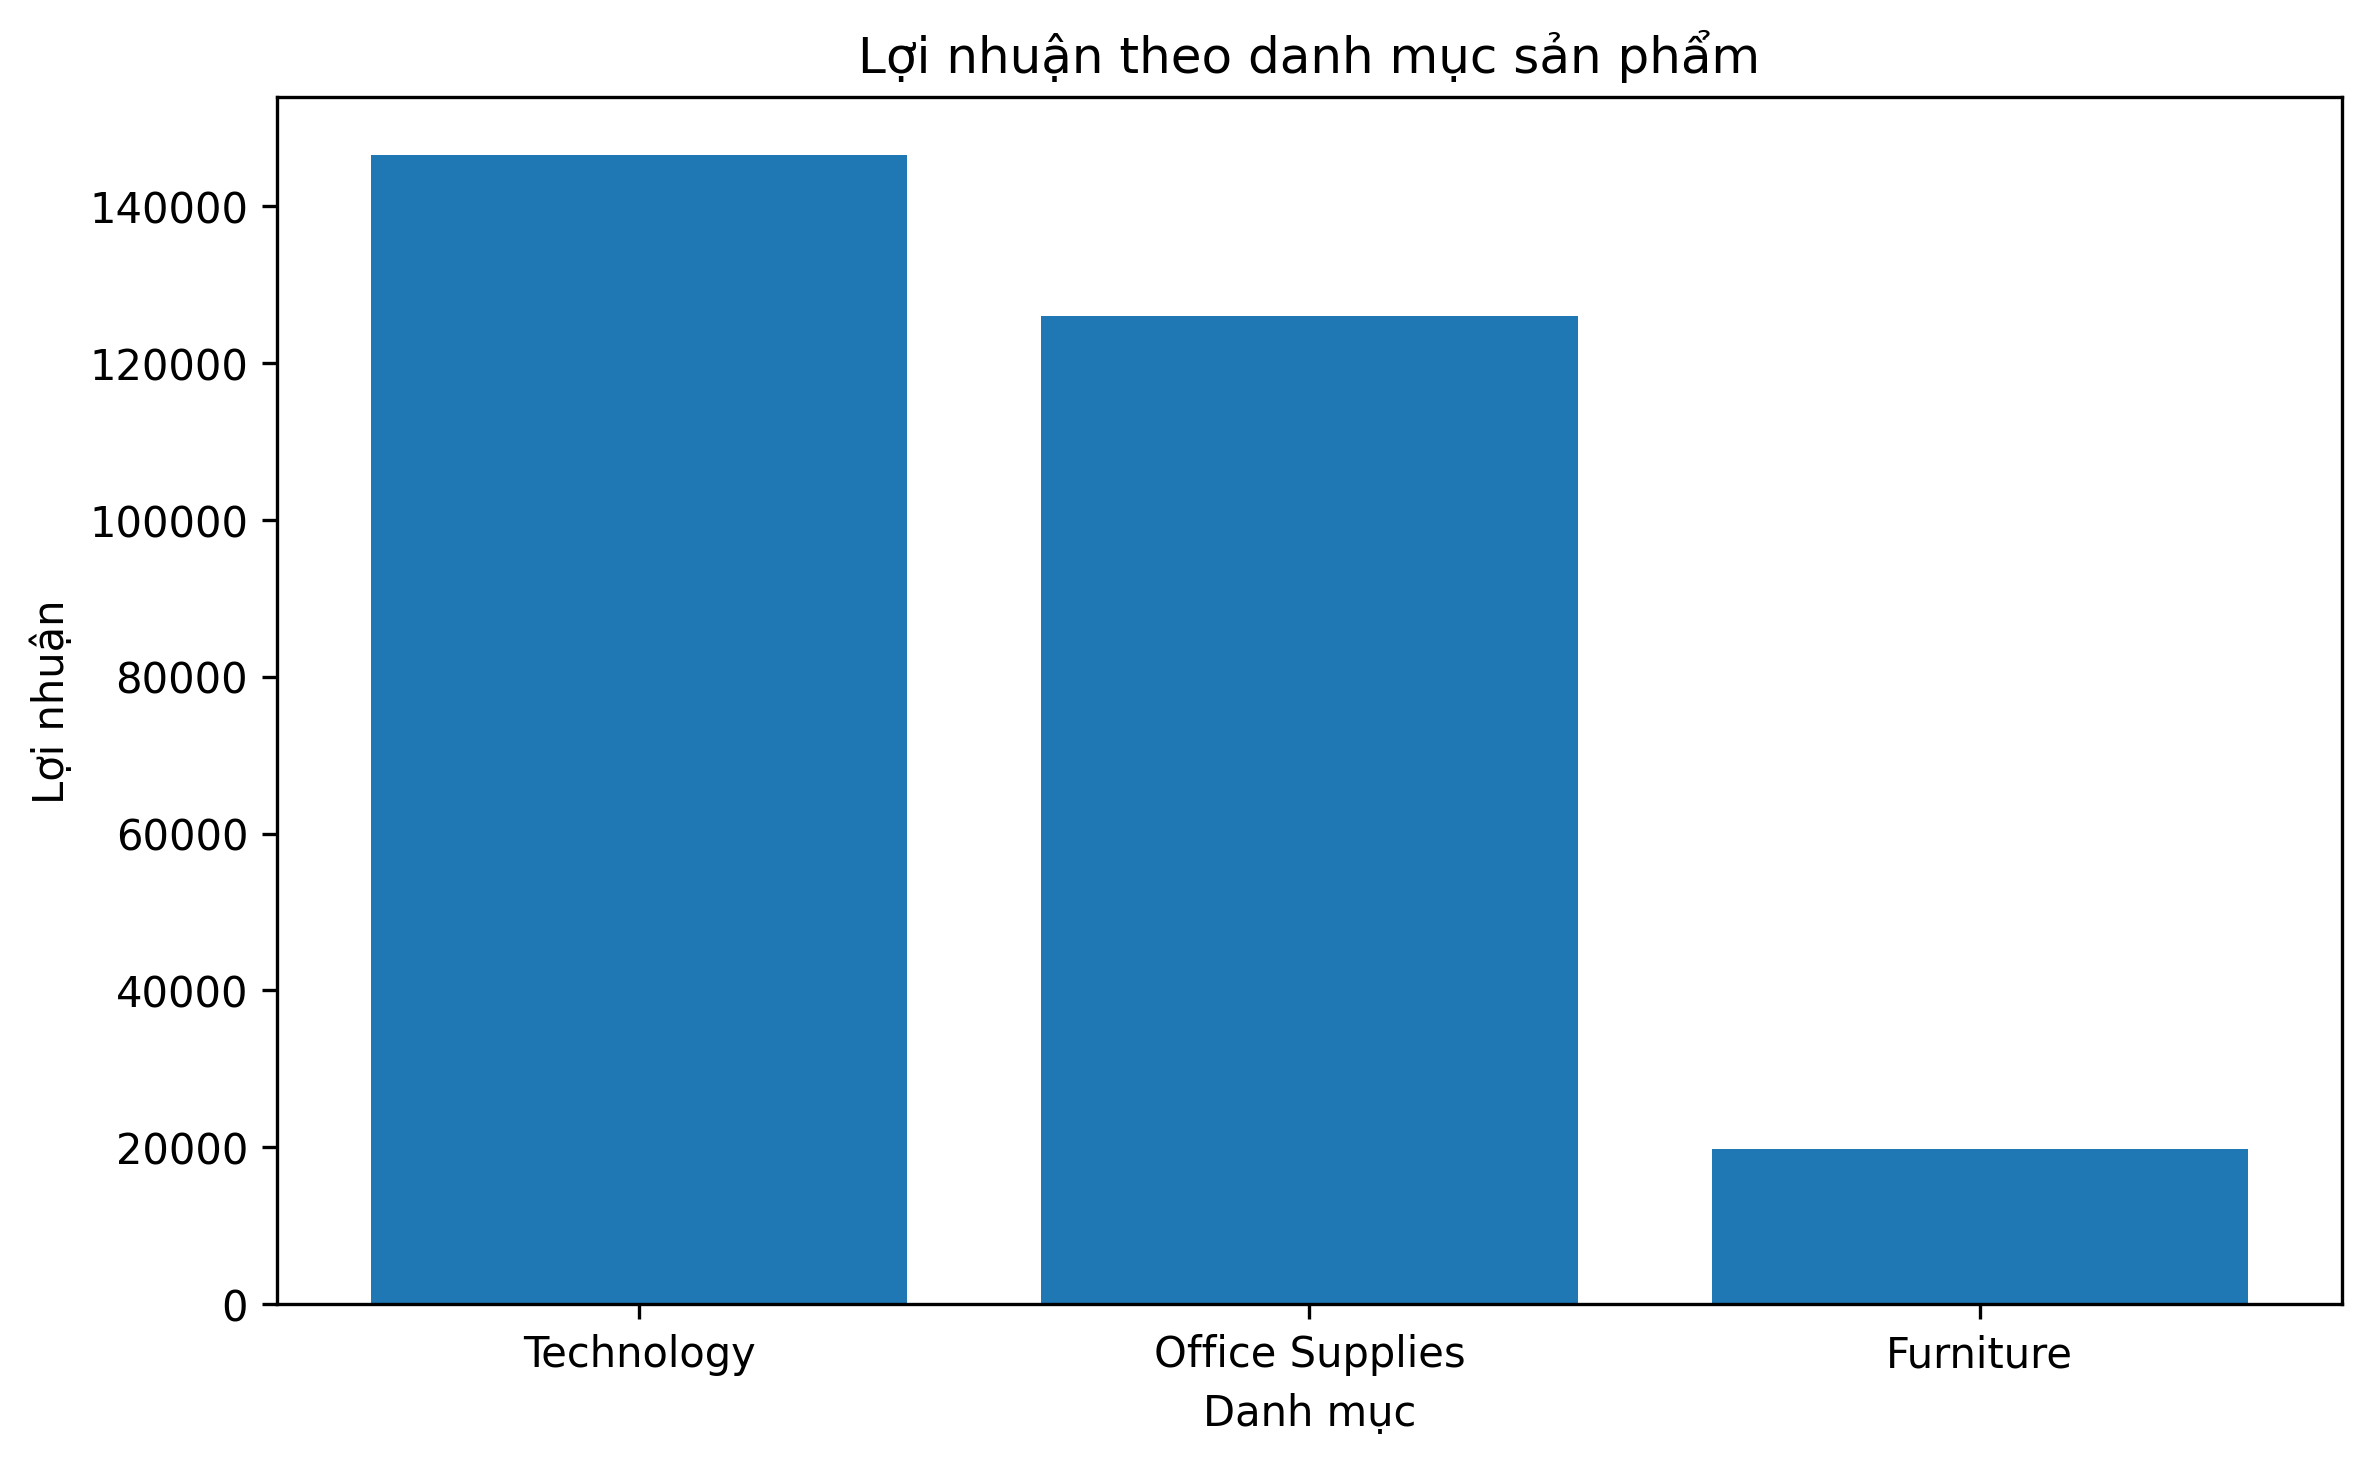
\includegraphics[width=0.85\textwidth]{images/anh_chuong3/hinh_3_3_loi_nhuan_theo_danh_muc.png}
\caption{Lợi nhuận theo danh mục sản phẩm}
\label{fig:loi-nhuan-danh-muc}
\end{figure}

Ở cấp tiểu danh mục, Copiers, Phones, Accessories và Paper là những nhóm có lợi nhuận cao. Ngược lại, Tables, Bookcases và Supplies là các tiểu danh mục có lợi nhuận âm. Đây là thông tin quan trọng để đánh giá hiệu quả kinh doanh theo từng nhóm sản phẩm cụ thể.

\begin{table}[H]
\centering
\caption{Top 5 tiểu danh mục có lợi nhuận cao nhất}
\label{tab:top-subcategory}
\begin{tabular}{|l|r|r|}
\hline
\textbf{Tiểu danh mục} & \textbf{Doanh thu} & \textbf{Lợi nhuận} \\
\hline
Copiers & 150.745,29 & 56.093,94 \\
\hline
Phones & 331.842,64 & 45.050,83 \\
\hline
Accessories & 167.380,32 & 41.936,64 \\
\hline
Paper & 79.540,54 & 34.511,51 \\
\hline
Binders & 207.354,88 & 31.426,10 \\
\hline
\end{tabular}
\end{table}

\begin{figure}[H]
\centering
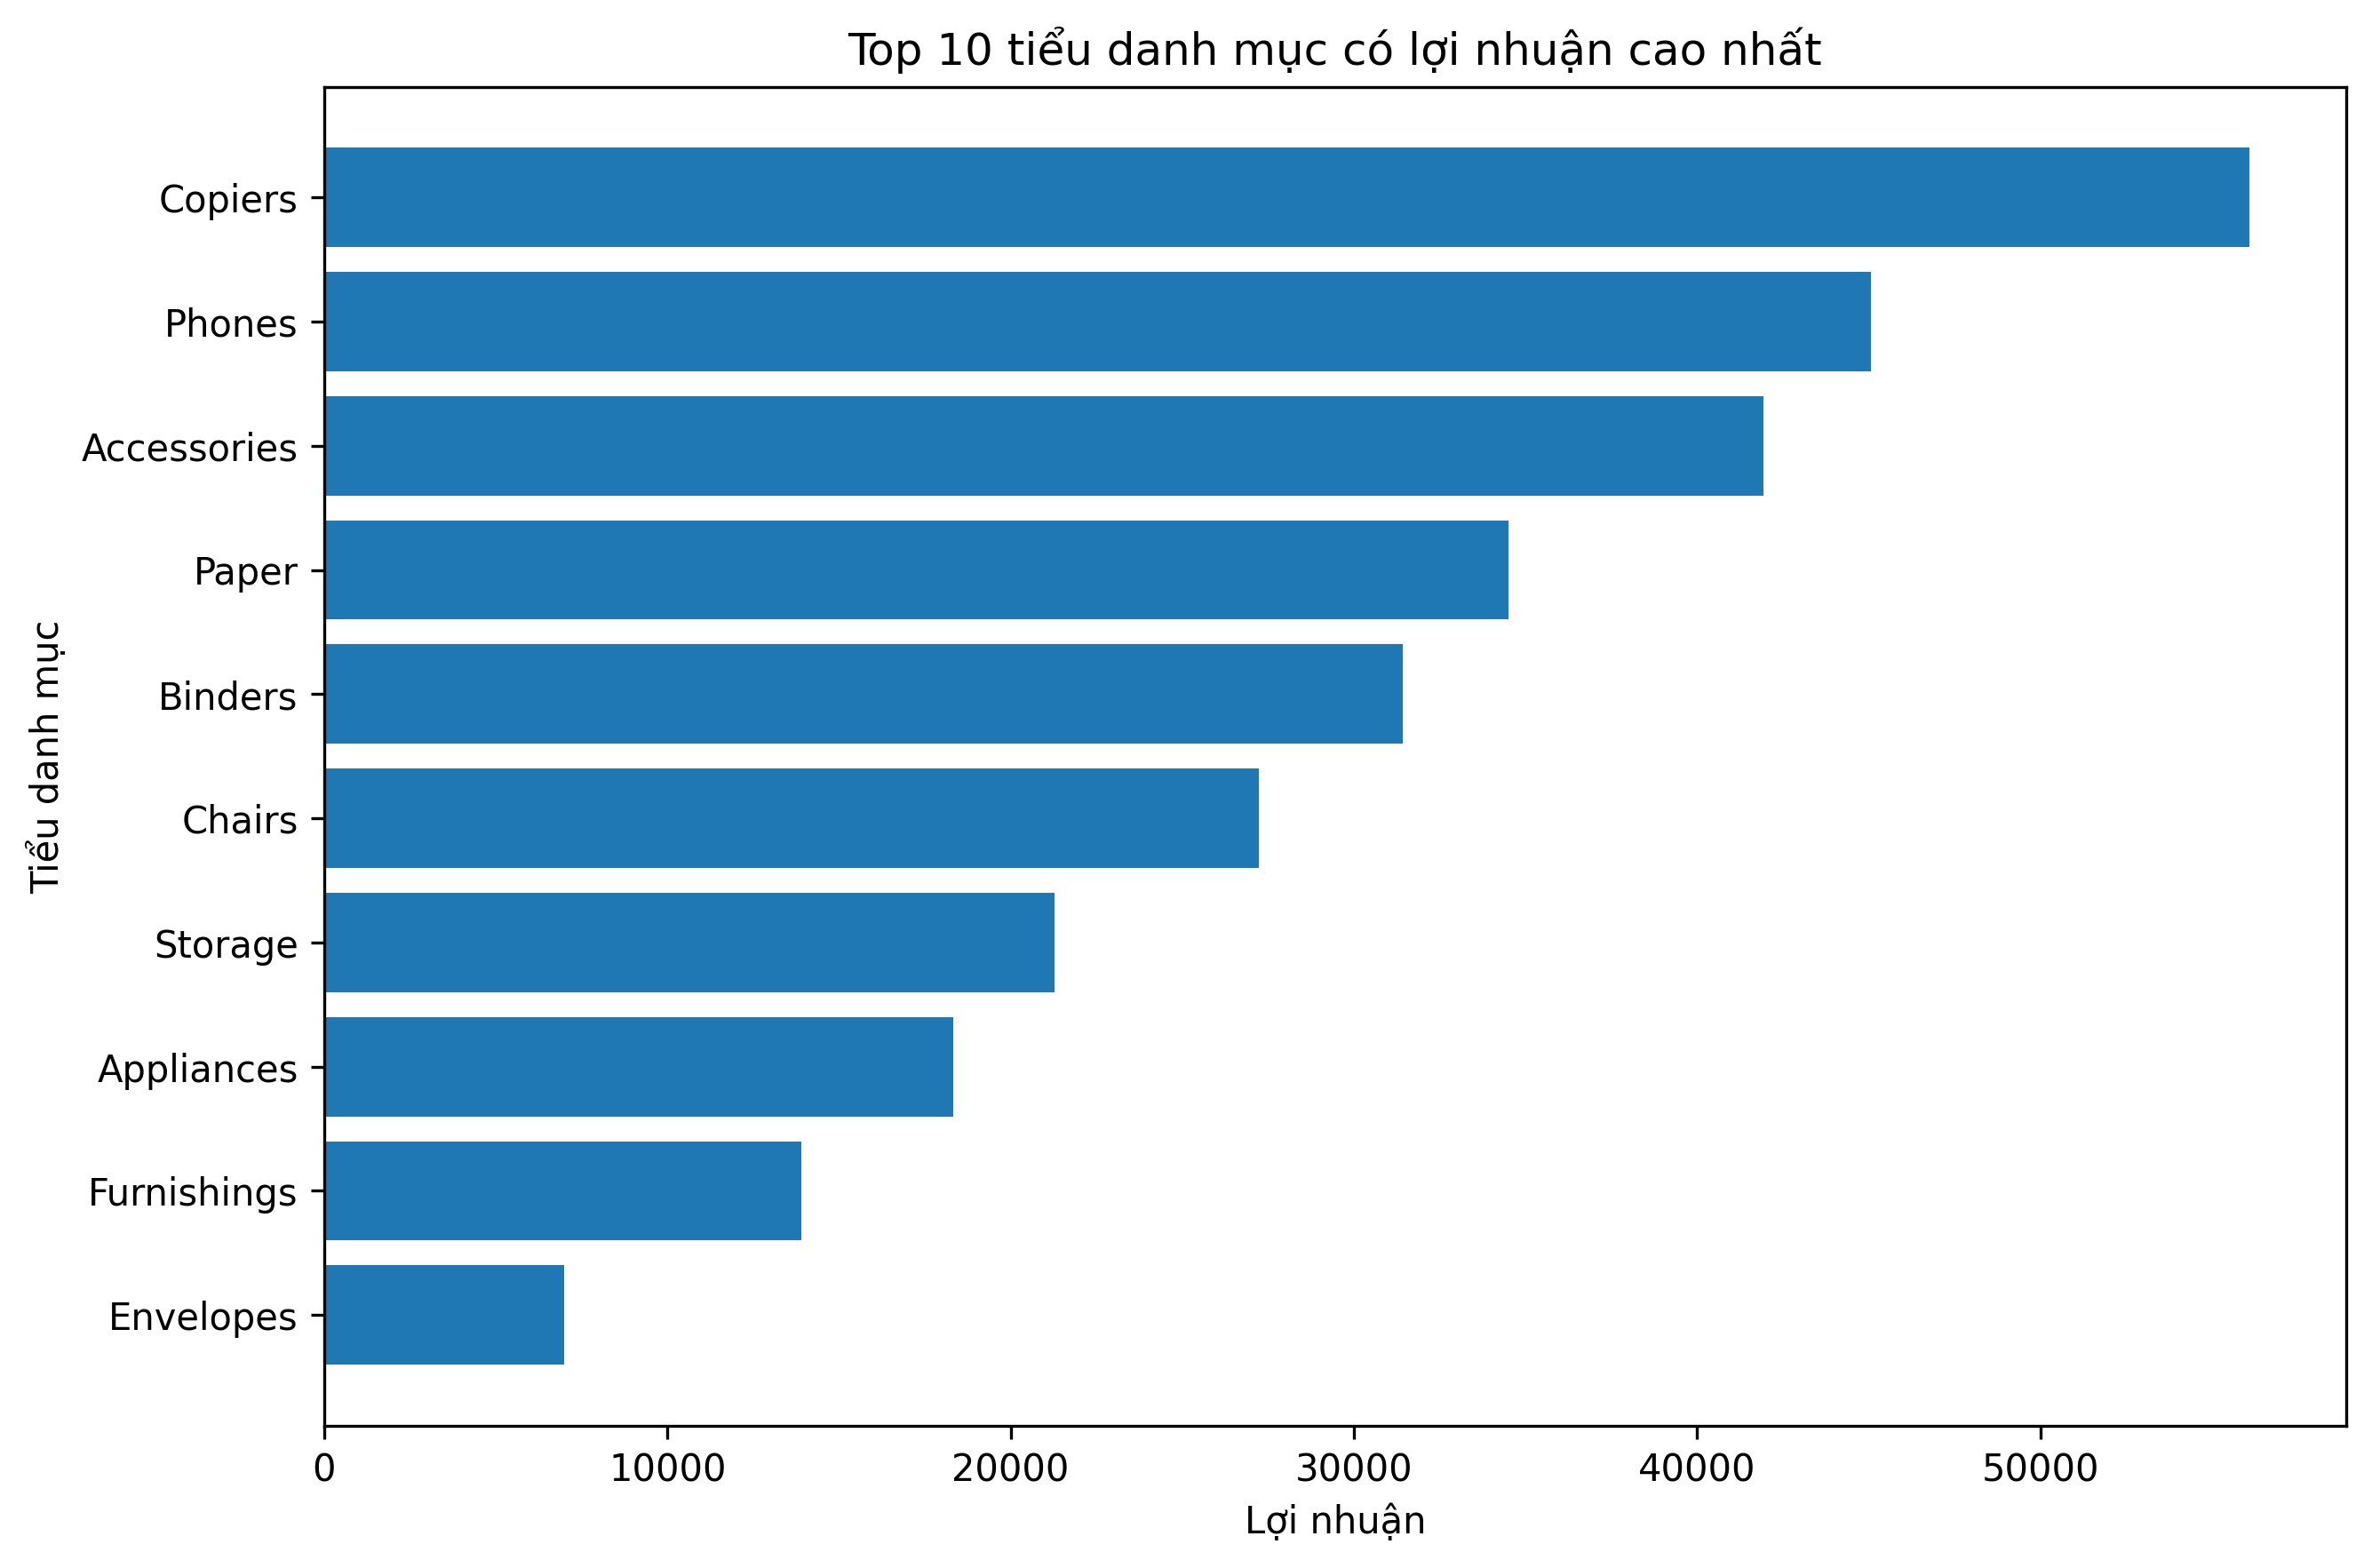
\includegraphics[width=0.9\textwidth]{images/anh_chuong3/hinh_3_4_top_10_tieu_danh_muc_loi_nhuan.png}
\caption{Top 10 tiểu danh mục có lợi nhuận cao nhất}
\label{fig:top-subcategory}
\end{figure}

\refstepcounter{subsection}
\subsection*{\thesubsection\quad Phân tích theo phân khúc khách hàng}

Phân khúc khách hàng là biến quan trọng để nhận diện xu hướng tiêu dùng của từng nhóm đối tượng. Kết quả tổng hợp cho thấy nhóm Consumer đóng góp doanh thu cao nhất với 1.170.660,25 và lợi nhuận cao nhất với 136.371,45. Nhóm Corporate đứng thứ hai, trong khi Home Office có quy mô doanh thu nhỏ hơn nhưng vẫn tạo ra lợi nhuận đáng kể.

\begin{table}[H]
\centering
\caption{Doanh thu và lợi nhuận theo phân khúc khách hàng}
\label{tab:phan-khuc}
\begin{tabular}{|l|r|r|r|r|}
\hline
\textbf{Phân khúc} & \textbf{Doanh thu} & \textbf{Lợi nhuận} & \textbf{Số đơn hàng} & \textbf{Số khách hàng} \\
\hline
Consumer & 1.170.660,25 & 136.371,45 & 2.628 & 416 \\
\hline
Corporate & 715.806,12 & 94.249,64 & 1.552 & 239 \\
\hline
Home Office & 440.067,98 & 61.675,73 & 931 & 149 \\
\hline
\end{tabular}
\end{table}

\begin{figure}[H]
\centering
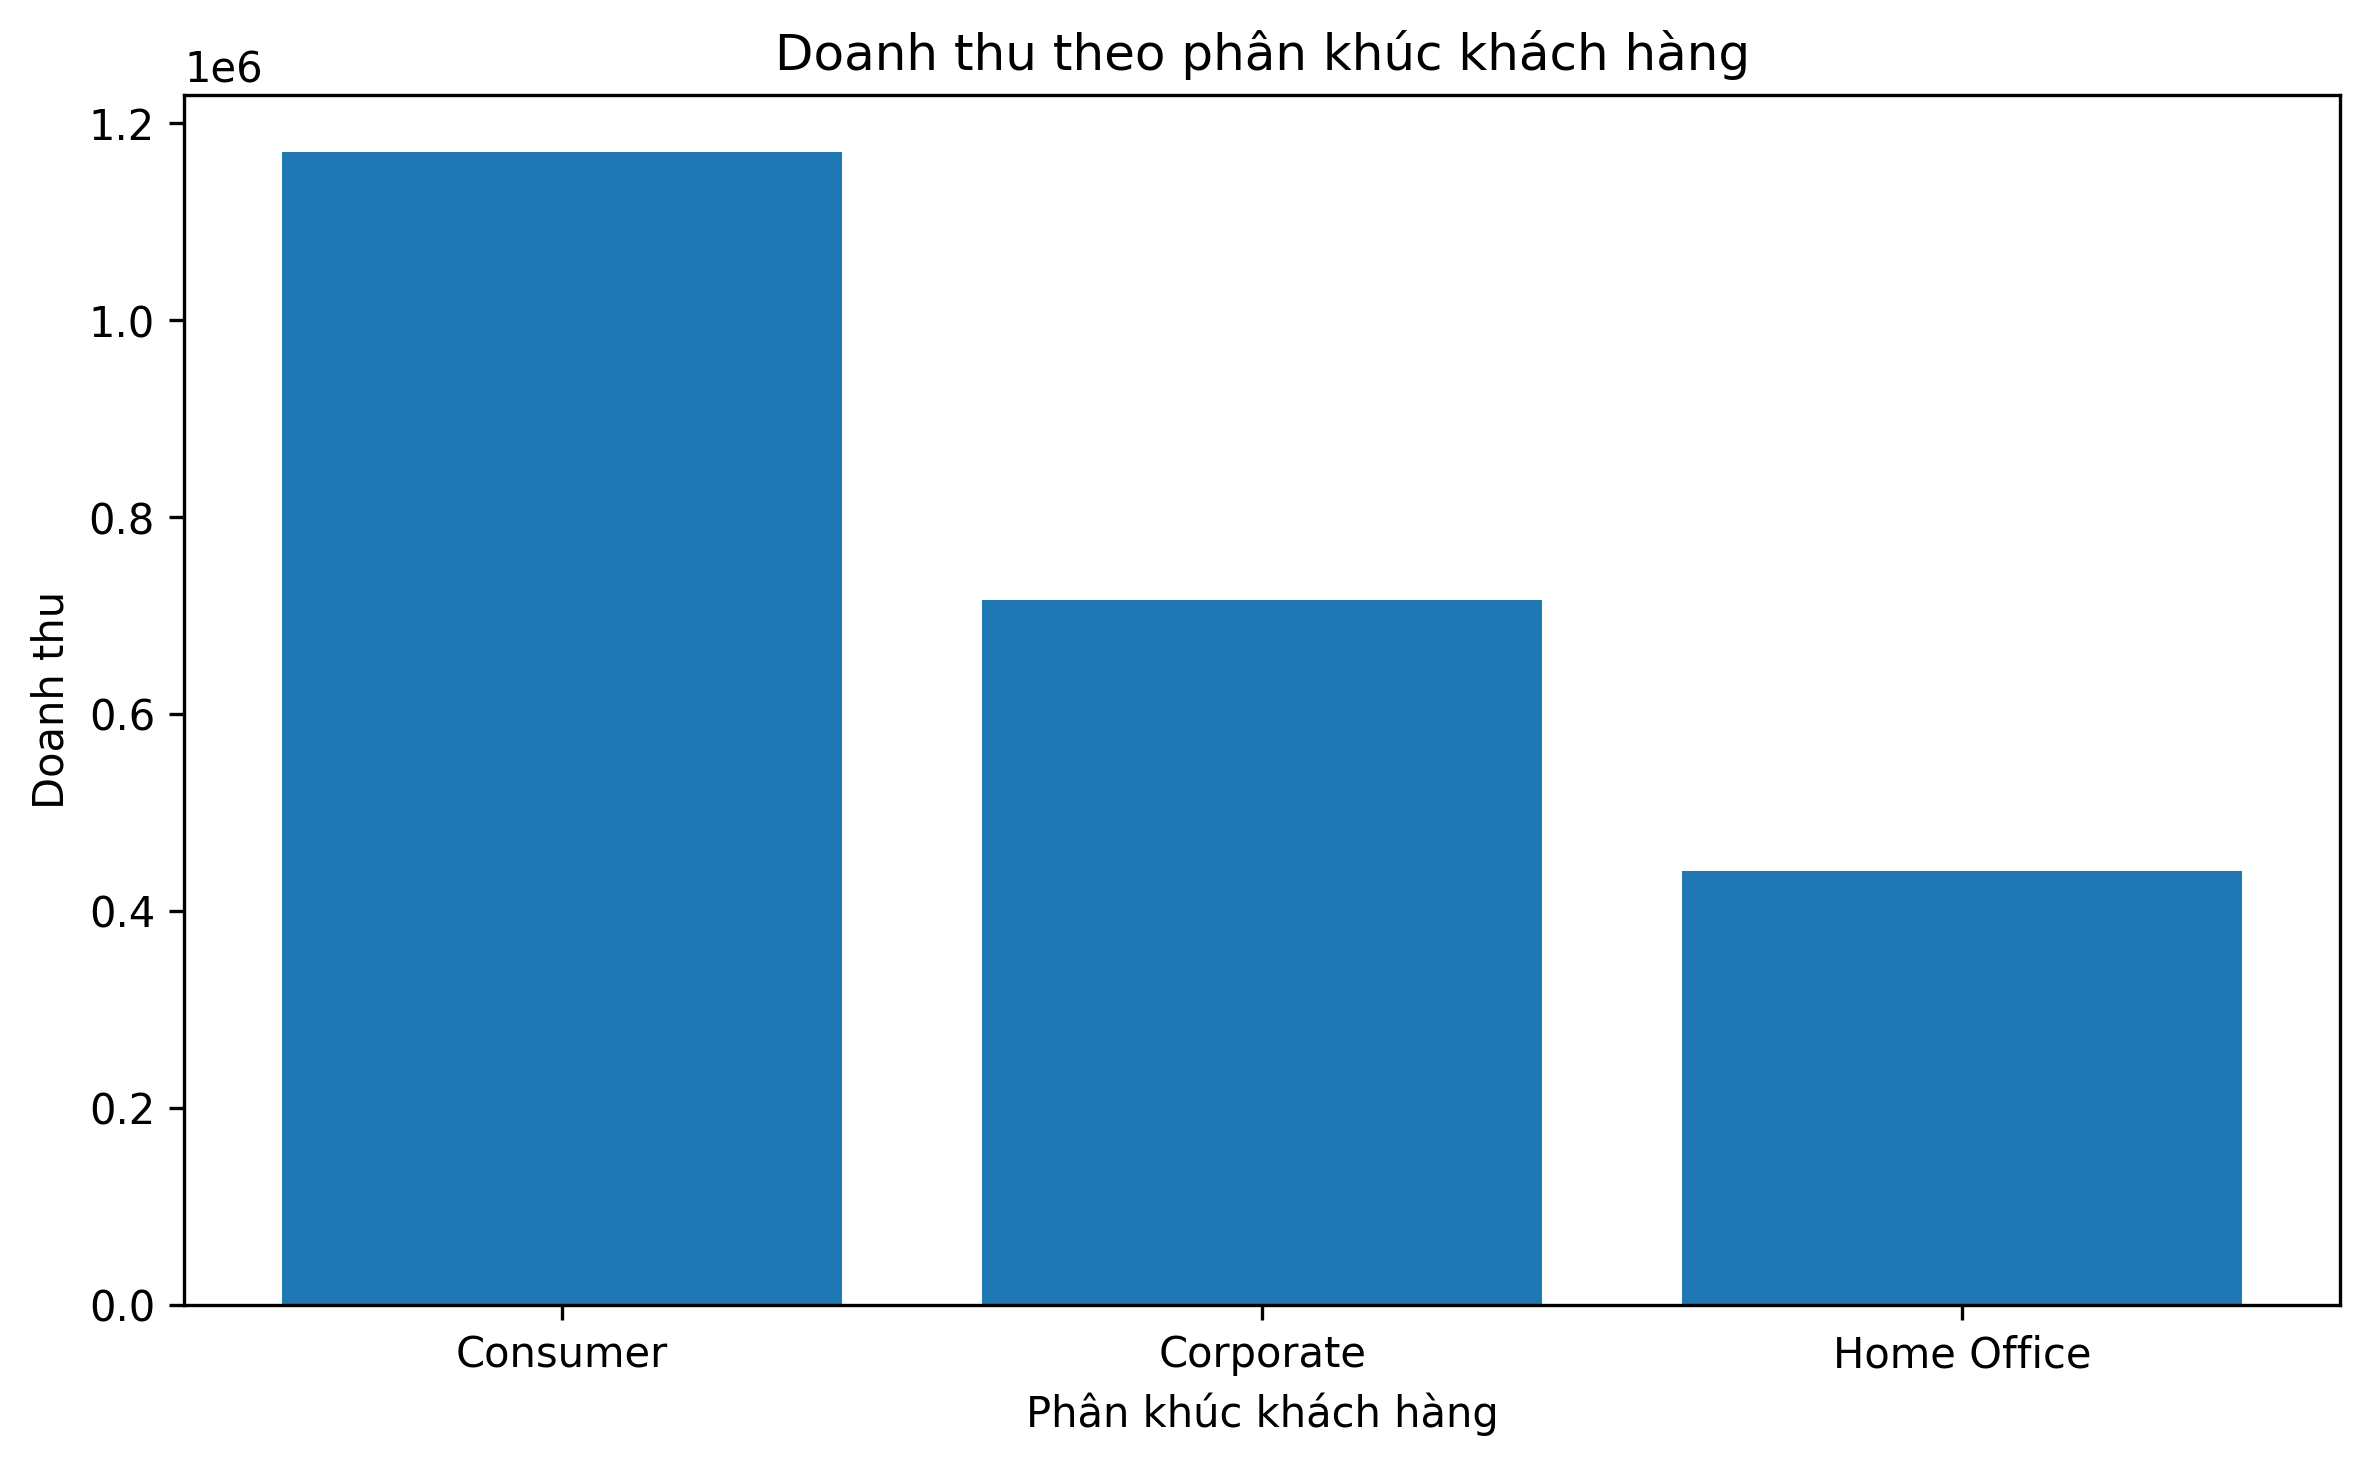
\includegraphics[width=0.85\textwidth]{images/anh_chuong3/hinh_3_5_doanh_thu_theo_phan_khuc.png}
\caption{Doanh thu theo phân khúc khách hàng}
\label{fig:doanh-thu-phan-khuc}
\end{figure}

Kết quả này cho thấy nhóm Consumer là nhóm khách hàng có xu hướng tiêu dùng cao nhất xét theo tổng doanh thu. Tuy nhiên, để đánh giá sâu hơn giá trị của từng nhóm khách hàng, cần kết hợp thêm các chỉ tiêu như lợi nhuận, số đơn hàng, giá trị trung bình mỗi đơn hàng và tần suất mua hàng.

\refstepcounter{subsection}
\subsection*{\thesubsection\quad Phân tích ảnh hưởng của chiết khấu đến lợi nhuận}

Chiết khấu là một yếu tố quan trọng trong hoạt động bán hàng vì có thể kích thích tiêu dùng nhưng đồng thời cũng làm giảm biên lợi nhuận. Vì vậy, việc phân tích mối quan hệ giữa chiết khấu và lợi nhuận giúp đánh giá hiệu quả của chính sách giảm giá. Theo kết quả tổng hợp, các nhóm chiết khấu thấp từ 0--20\% vẫn tạo ra lợi nhuận dương, trong khi các nhóm chiết khấu từ 20\% trở lên bắt đầu ghi nhận lợi nhuận âm ở nhiều mức khác nhau.

\begin{table}[H]
\centering
\caption{Lợi nhuận theo nhóm chiết khấu}
\label{tab:chiet-khau}
\begin{tabular}{|l|r|r|r|}
\hline
\textbf{Nhóm chiết khấu} & \textbf{Doanh thu} & \textbf{Lợi nhuận} & \textbf{Số dòng} \\
\hline
0--10\% & 1.160.275,60 & 335.818,56 & 5.021 \\
\hline
10--20\% & 801.497,85 & 92.498,94 & 3.758 \\
\hline
20--30\% & 104.474,07 & -10.513,45 & 230 \\
\hline
30--40\% & 130.991,18 & -25.477,51 & 234 \\
\hline
40--50\% & 64.403,51 & -22.999,54 & 77 \\
\hline
50--60\% & 7.105,94 & -6.164,35 & 149 \\
\hline
60--70\% & 40.805,27 & -40.300,57 & 424 \\
\hline
70--80\% & 16.980,15 & -30.565,27 & 301 \\
\hline
\end{tabular}
\end{table}

\begin{figure}[H]
\centering
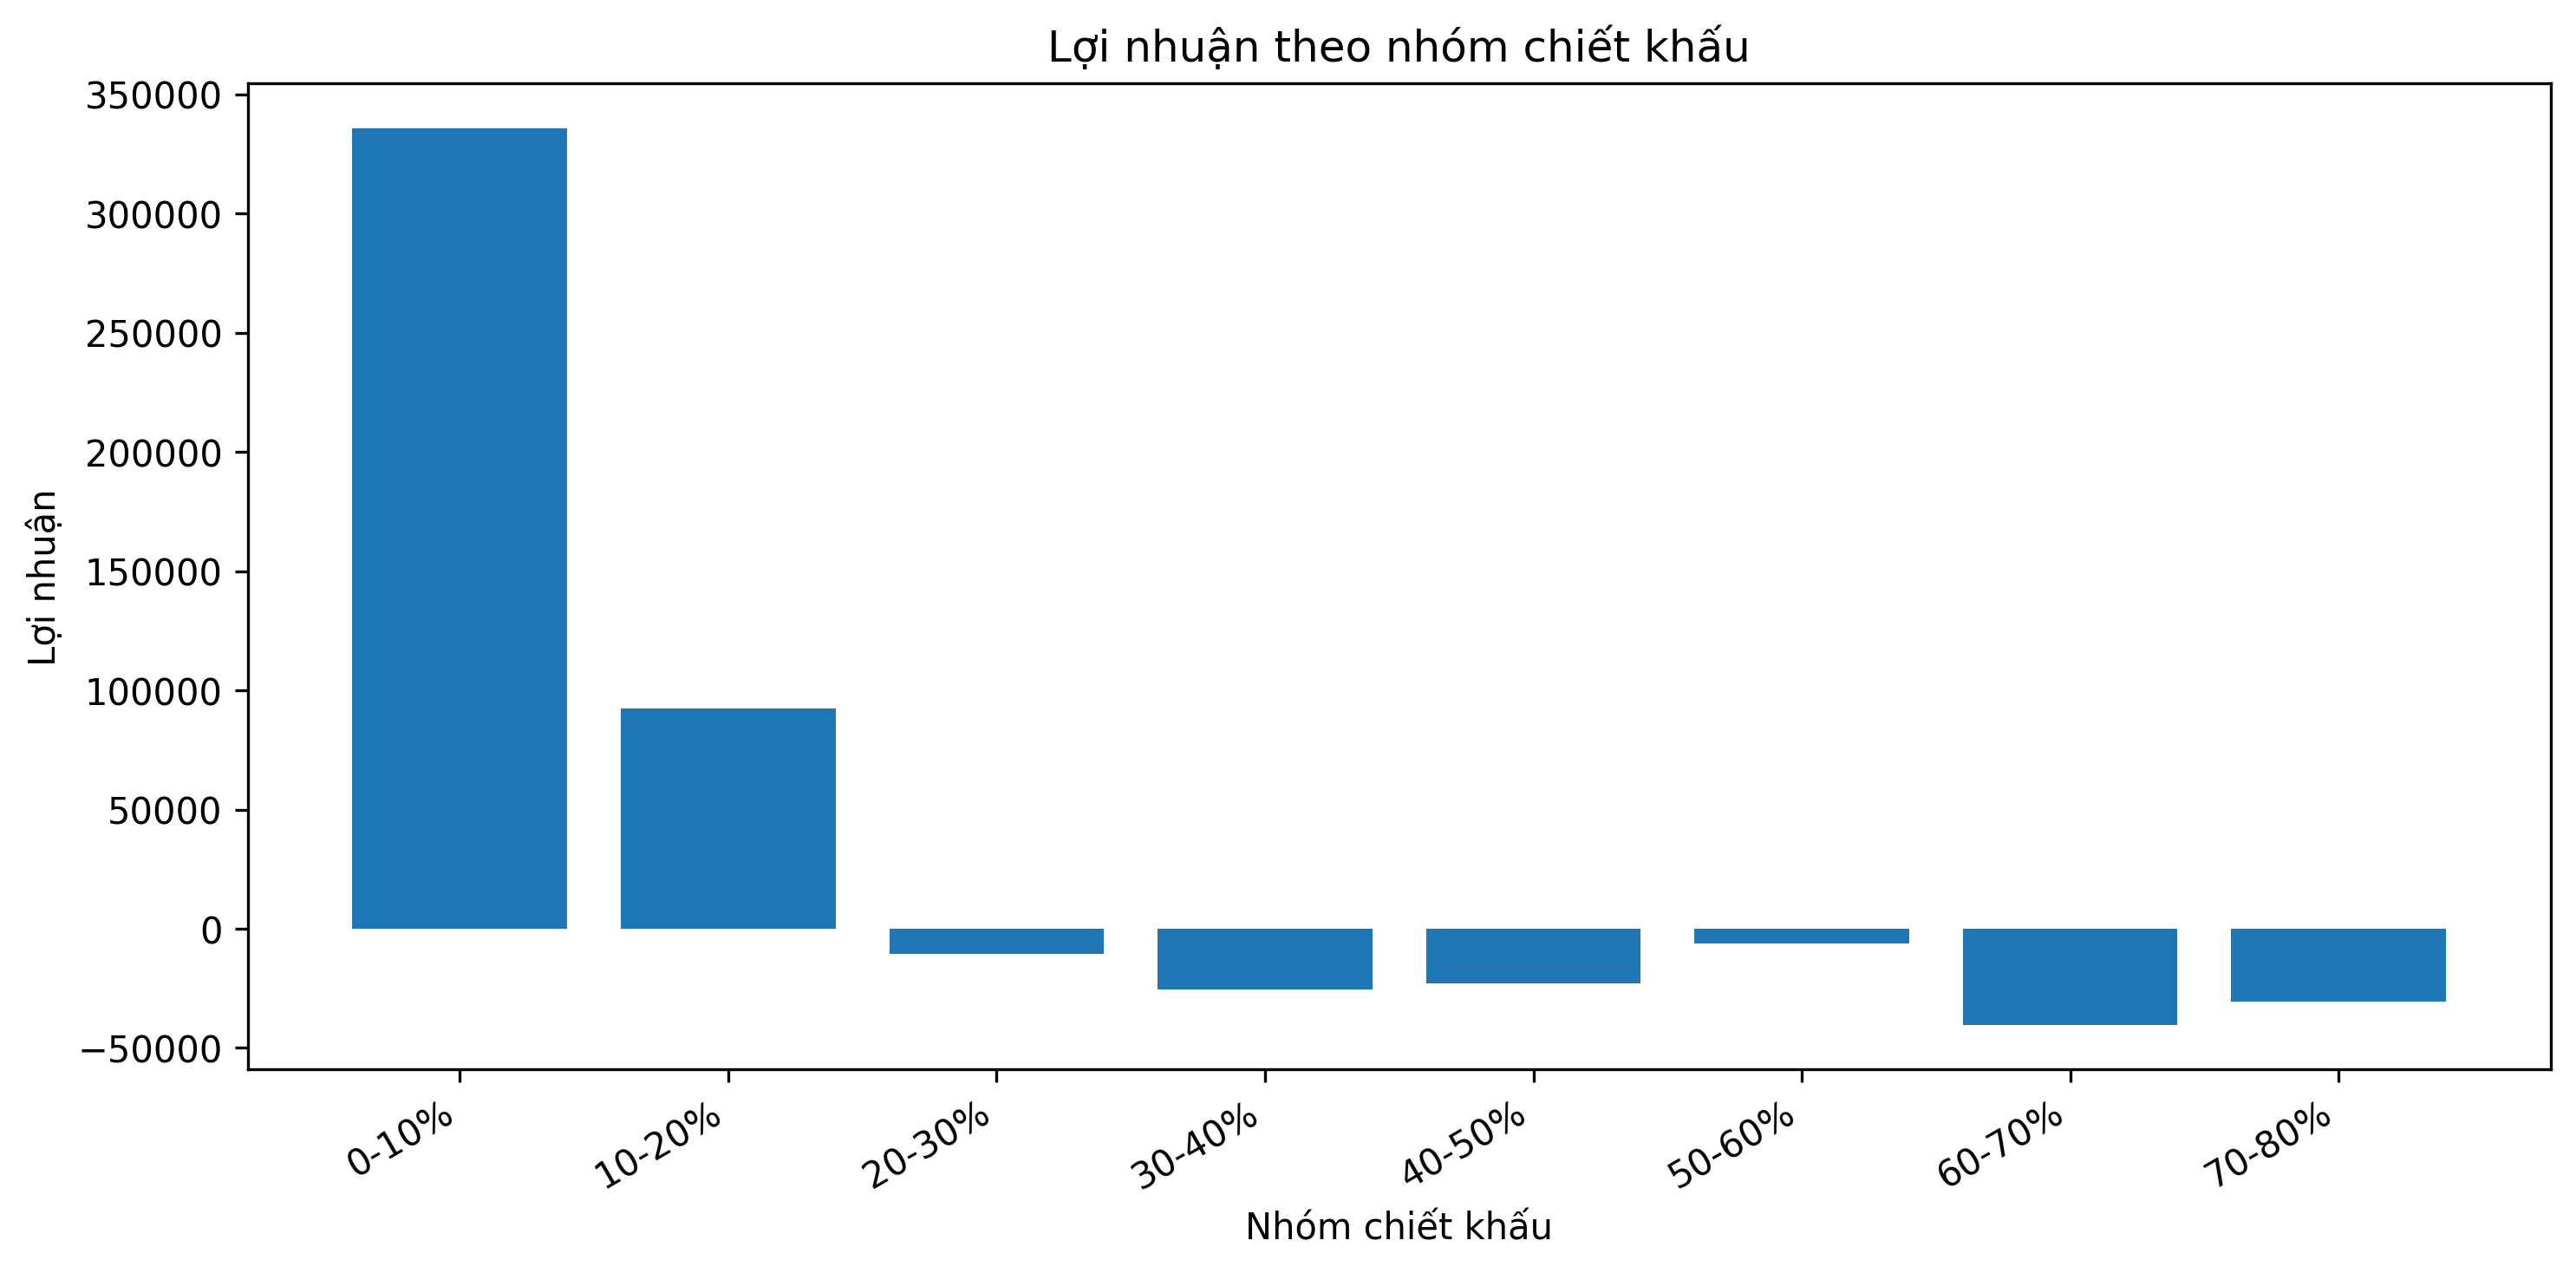
\includegraphics[width=0.9\textwidth]{images/anh_chuong3/hinh_3_6_loi_nhuan_theo_nhom_chiet_khau.png}
\caption{Lợi nhuận theo nhóm chiết khấu}
\label{fig:loi-nhuan-chiet-khau}
\end{figure}

Kết quả trên cho thấy chiết khấu cao có xu hướng làm giảm lợi nhuận, đặc biệt ở các nhóm từ 60--80\%. Đây là một insight quan trọng vì doanh nghiệp không chỉ cần quan tâm đến việc tăng doanh thu thông qua giảm giá mà còn phải kiểm soát tác động của chiết khấu đến hiệu quả sinh lời.

\section{Thiết kế và xây dựng dashboard trong Power BI}

\refstepcounter{subsection}
\subsection*{\thesubsection\quad Mục tiêu thiết kế dashboard}

Dashboard được xây dựng nhằm trực quan hóa các kết quả phân tích chính của bộ dữ liệu Superstore Sales, giúp tổng hợp các chỉ số quan trọng, biểu diễn dữ liệu dưới dạng biểu đồ và hỗ trợ người dùng theo dõi tình hình kinh doanh một cách trực quan. Trong đồ án này, dashboard được thiết kế với mục tiêu hỗ trợ trả lời các câu hỏi nghiên cứu liên quan đến xu hướng doanh số, hiệu quả theo khu vực, theo danh mục sản phẩm, hành vi tiêu dùng của phân khúc khách hàng và ảnh hưởng của chiết khấu đến lợi nhuận.

Các chỉ tiêu chính được sử dụng trên dashboard gồm tổng doanh thu, tổng lợi nhuận, số lượng bán, số đơn hàng, số khách hàng, doanh thu theo thời gian, doanh thu và lợi nhuận theo khu vực, lợi nhuận theo danh mục sản phẩm, doanh thu theo phân khúc khách hàng và lợi nhuận theo mức chiết khấu.

\refstepcounter{subsection}
\subsection*{\thesubsection\quad Cấu trúc dashboard}

Dashboard Power BI được tổ chức thành ba trang chính nhằm bảo đảm nội dung phân tích có tính hệ thống và dễ theo dõi:

\begin{itemize}
    \item \textbf{Trang 1: Tổng quan kinh doanh.} Trang này tập trung vào các chỉ số tổng quan như tổng doanh thu, tổng lợi nhuận, số lượng bán, số đơn hàng và xu hướng doanh thu theo thời gian.
    \item \textbf{Trang 2: Khu vực và sản phẩm.} Trang này phân tích doanh thu, lợi nhuận theo khu vực, danh mục và tiểu danh mục sản phẩm, từ đó hỗ trợ nhận diện khu vực và nhóm sản phẩm hoạt động hiệu quả.
    \item \textbf{Trang 3: Khách hàng và chiết khấu.} Trang này tập trung phân tích doanh thu theo phân khúc khách hàng và ảnh hưởng của chiết khấu đến lợi nhuận.
\end{itemize}

\begin{figure}[H]
\centering
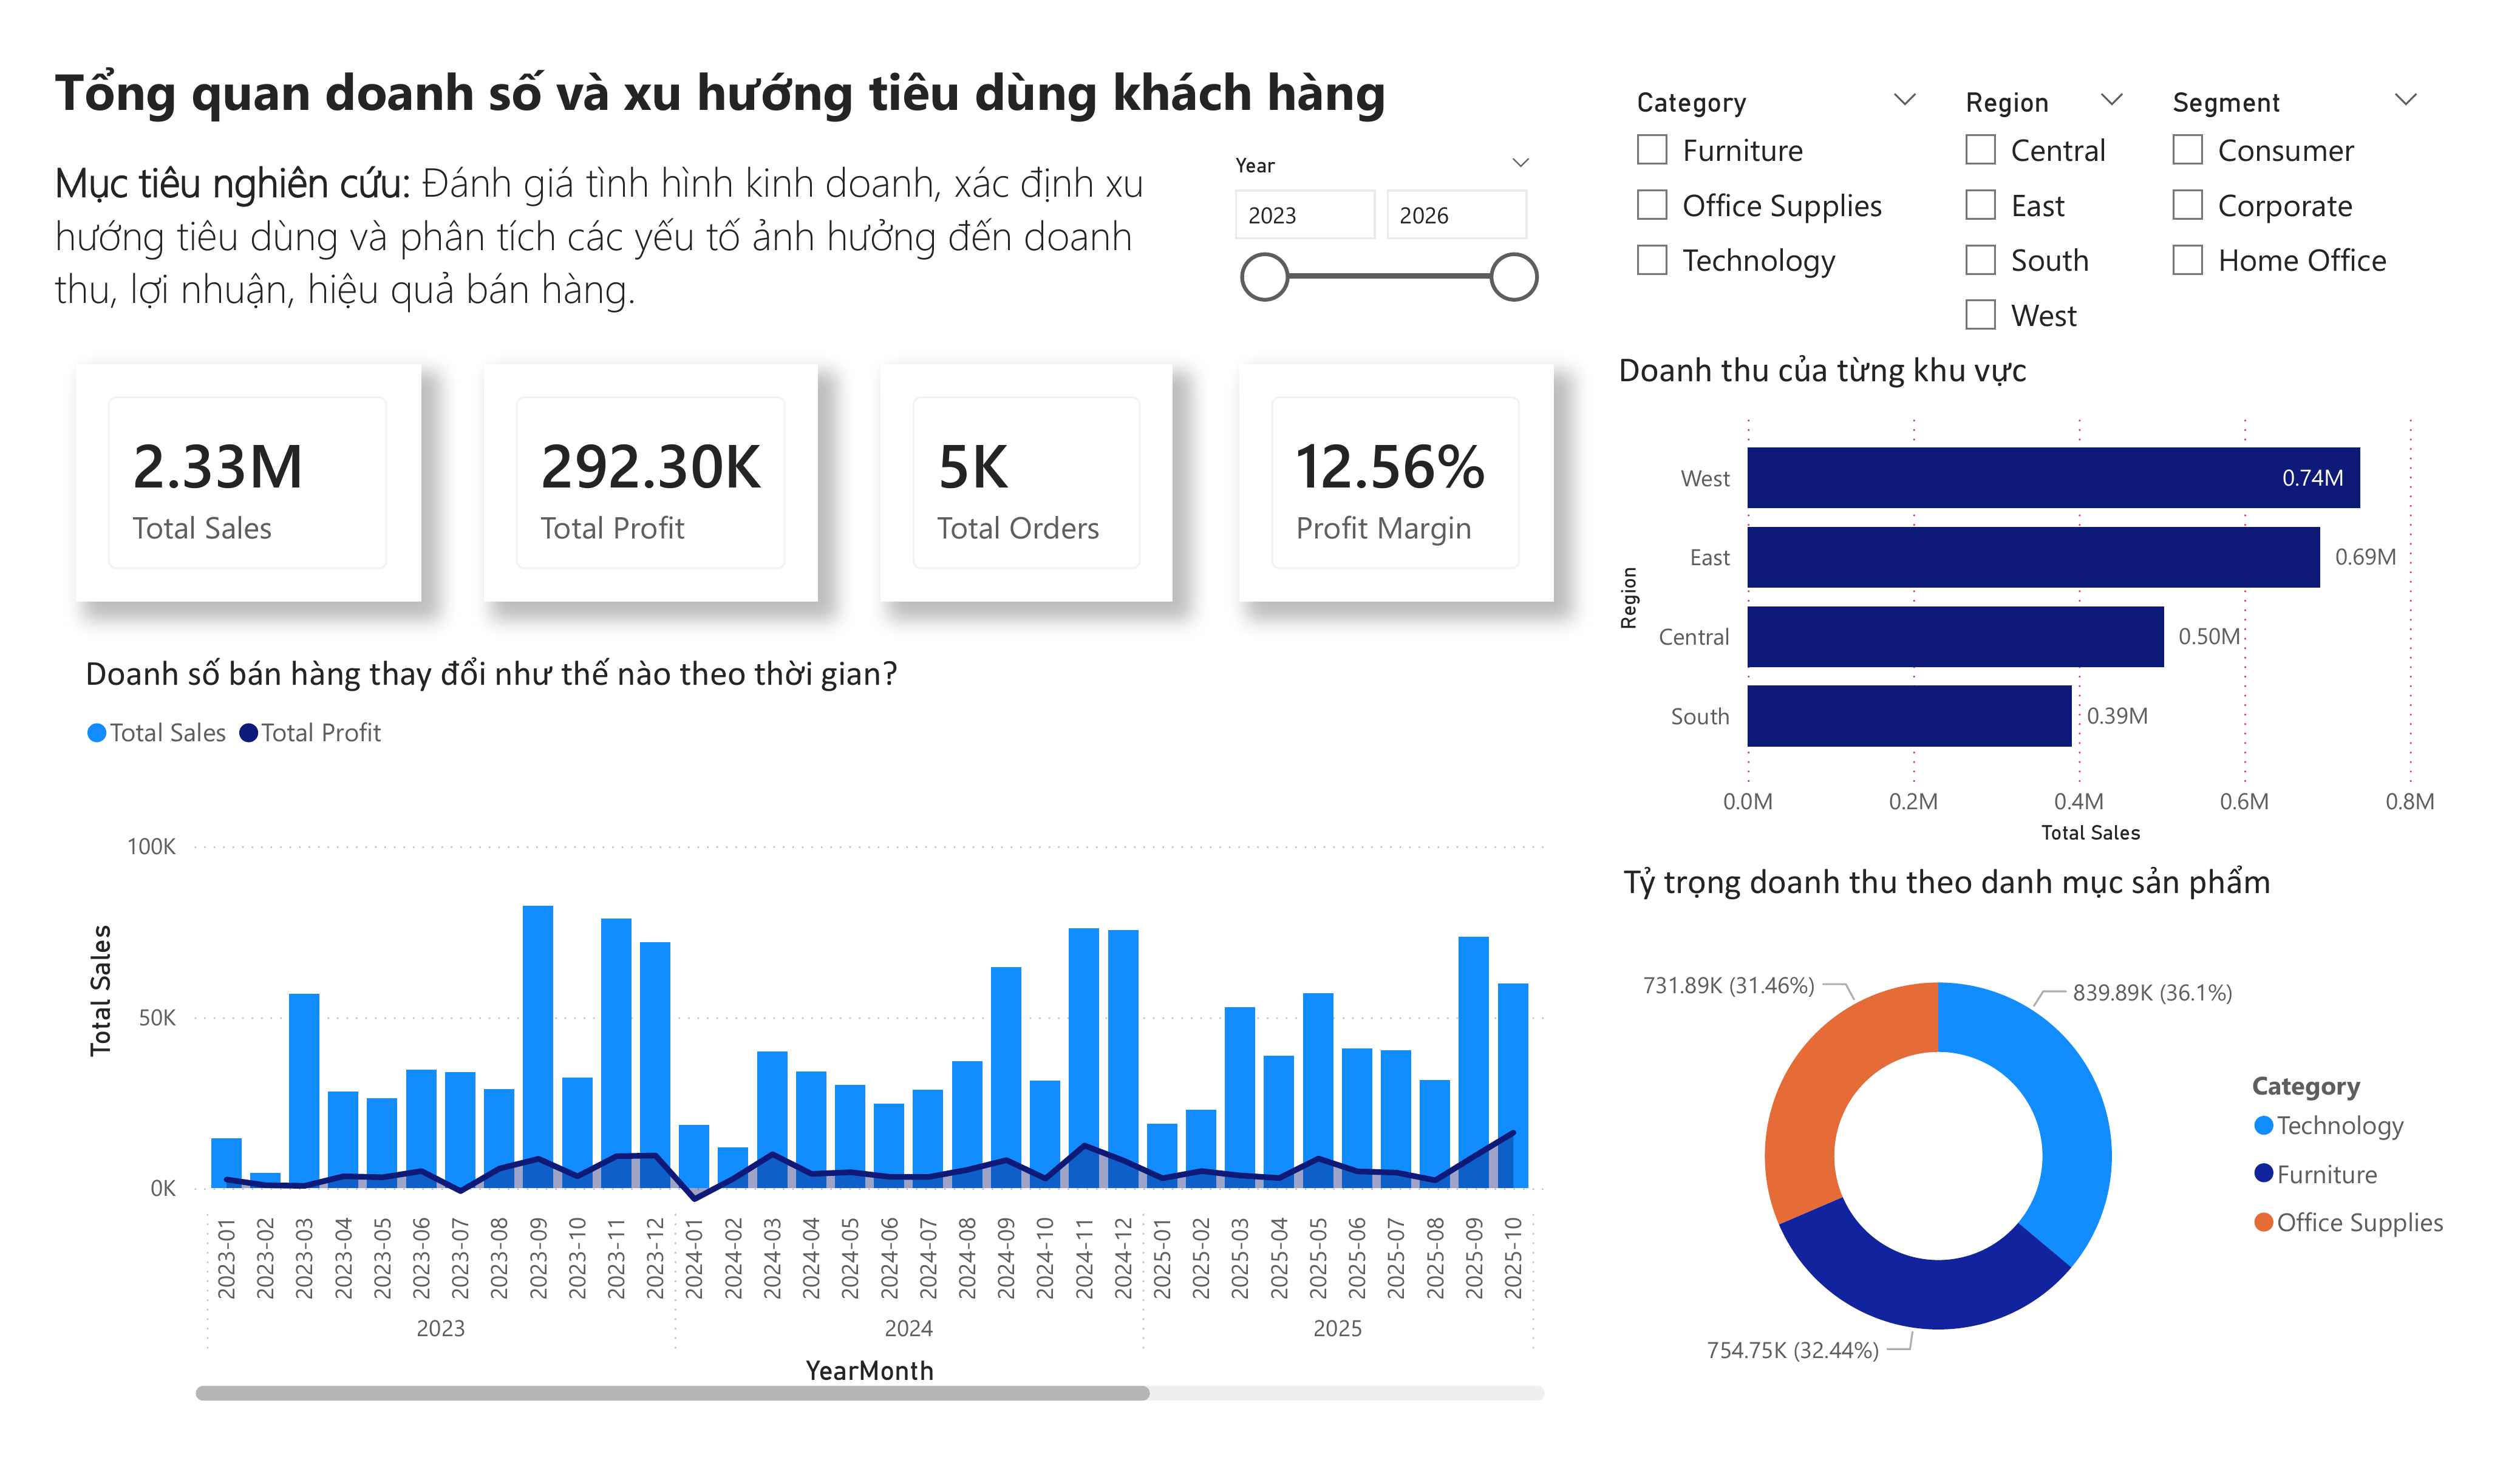
\includegraphics[width=0.95\textwidth]{images/anh_chuong3/dashboard_tong_quan_kinh_doanh.png}
\caption{Trang tổng quan kinh doanh trên Power BI}
\label{fig:dashboard-tong-quan}
\end{figure}

\begin{figure}[H]
\centering
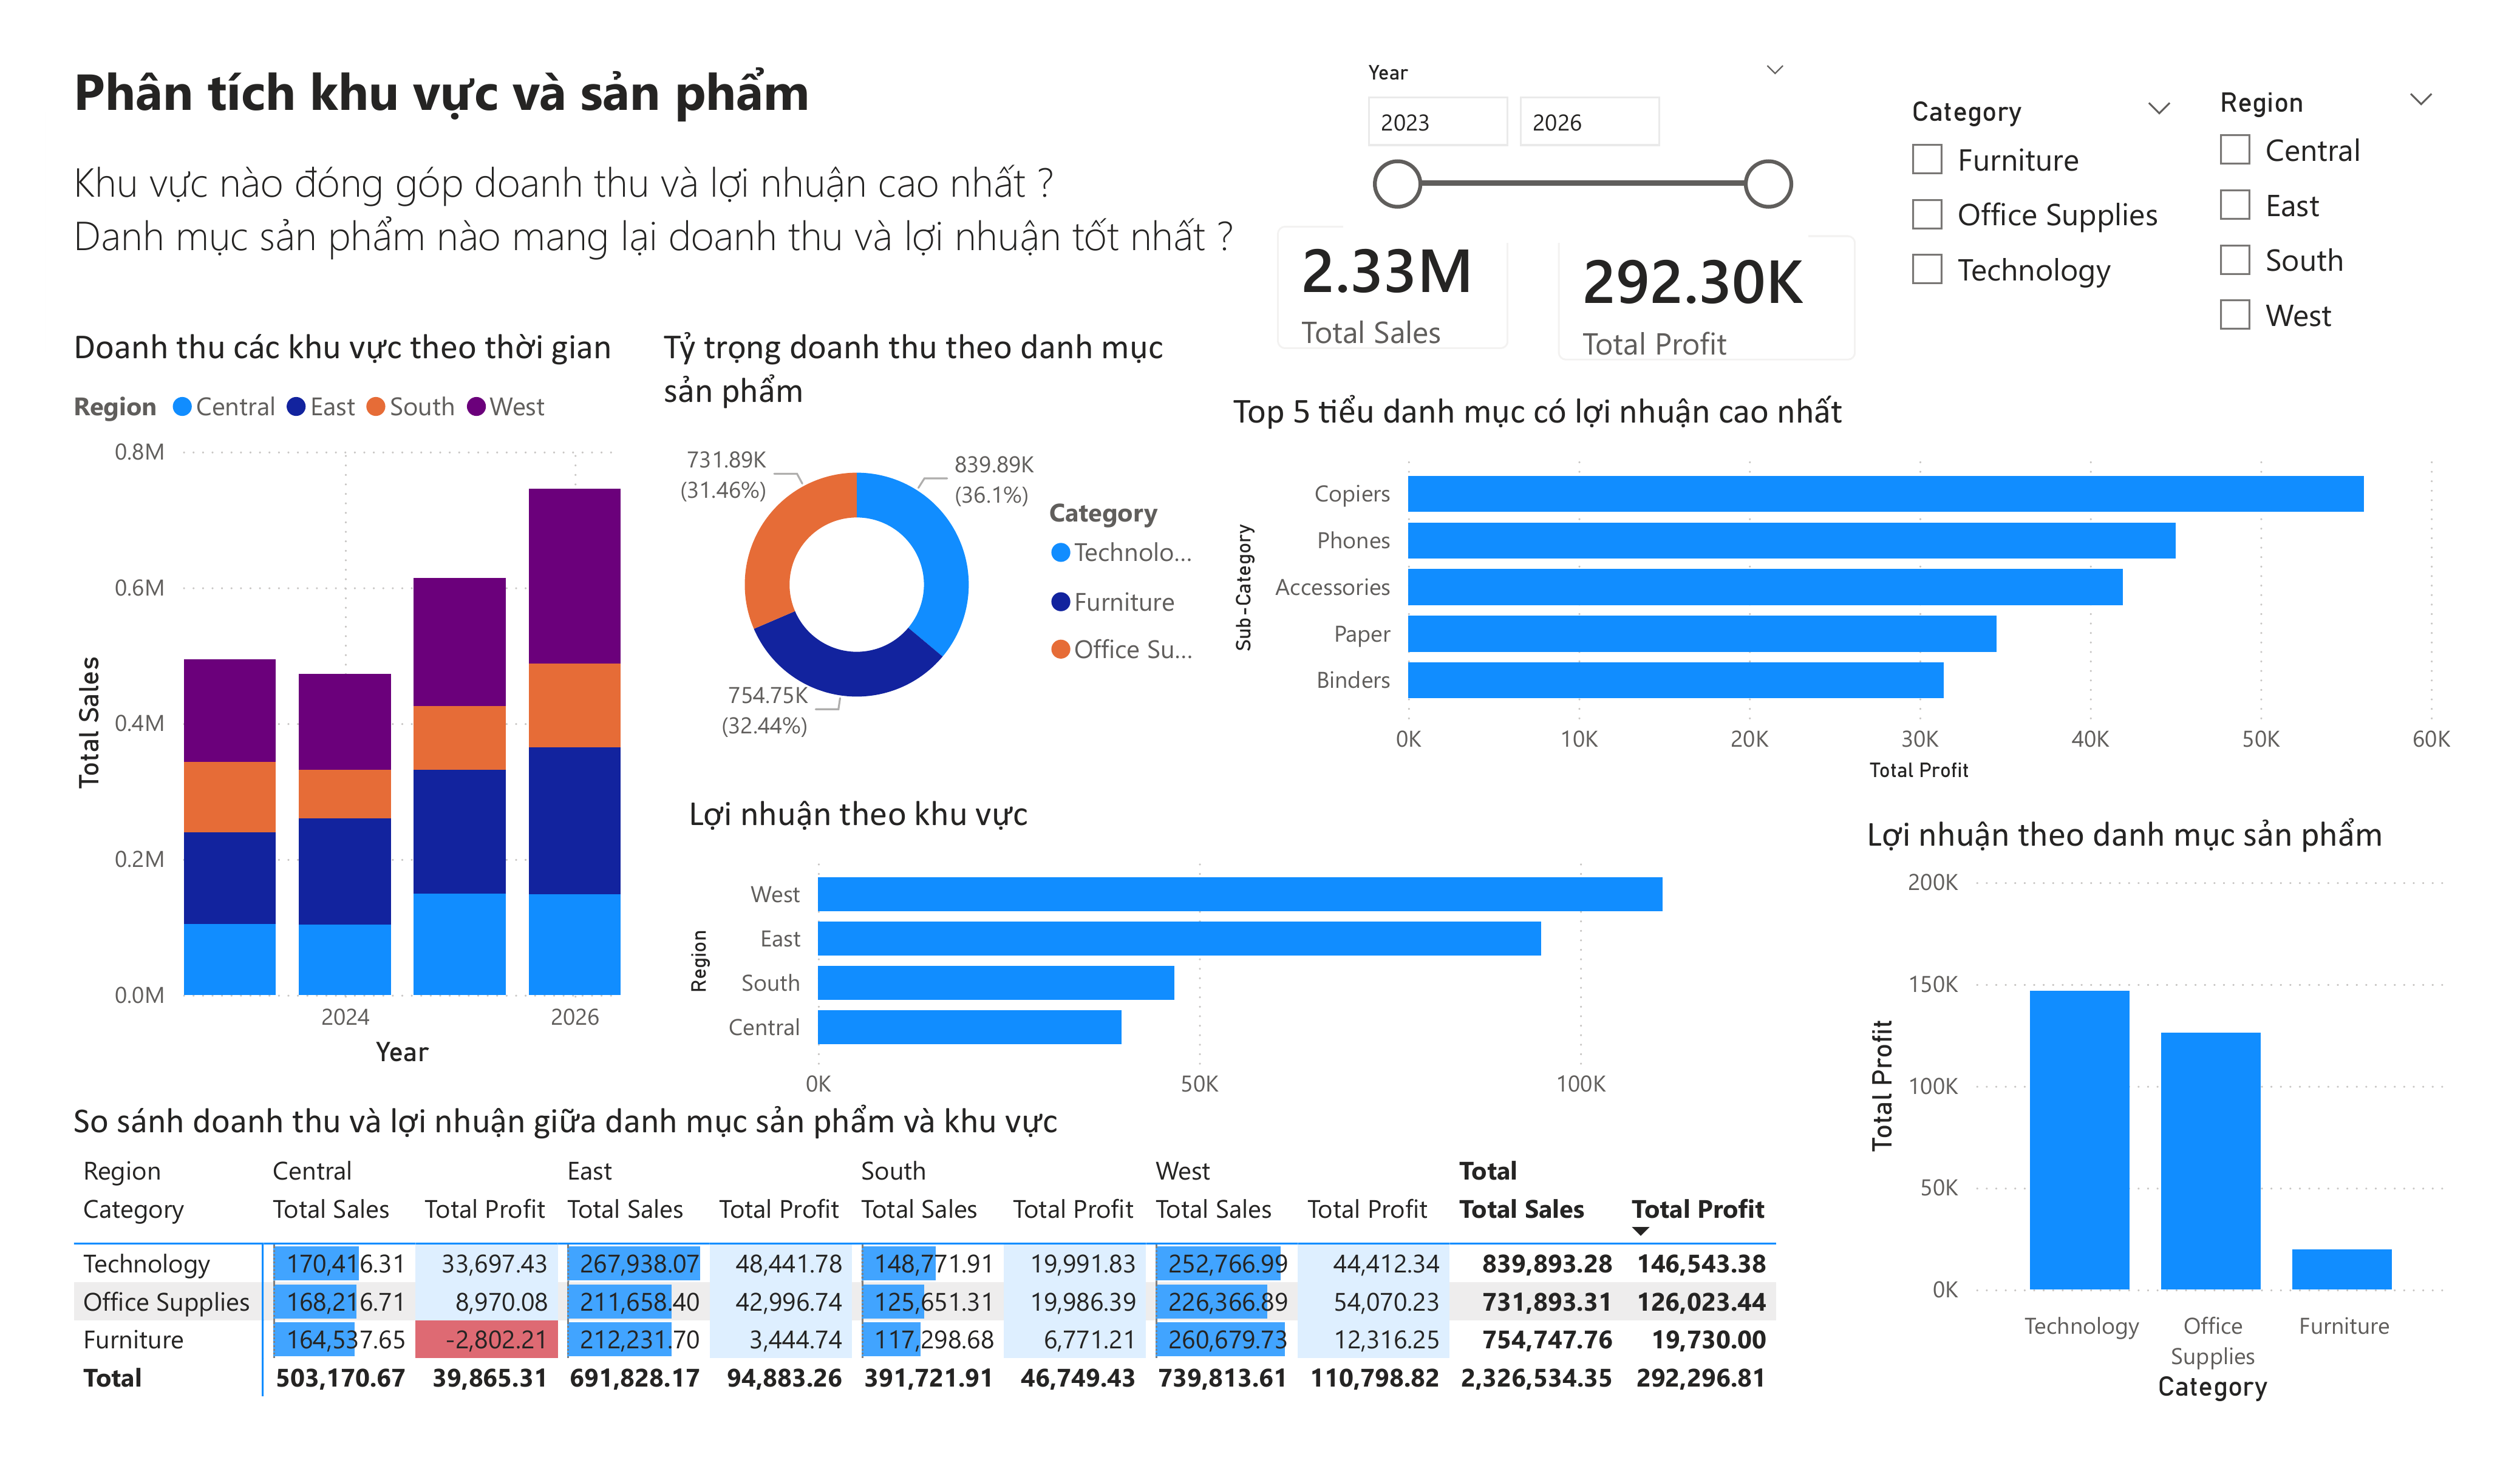
\includegraphics[width=0.95\textwidth]{images/anh_chuong3/dashboard_khu_vuc_san_pham.png}
\caption{Trang phân tích khu vực và sản phẩm trên Power BI}
\label{fig:dashboard-khu-vuc-san-pham}
\end{figure}

\begin{figure}[H]
\centering
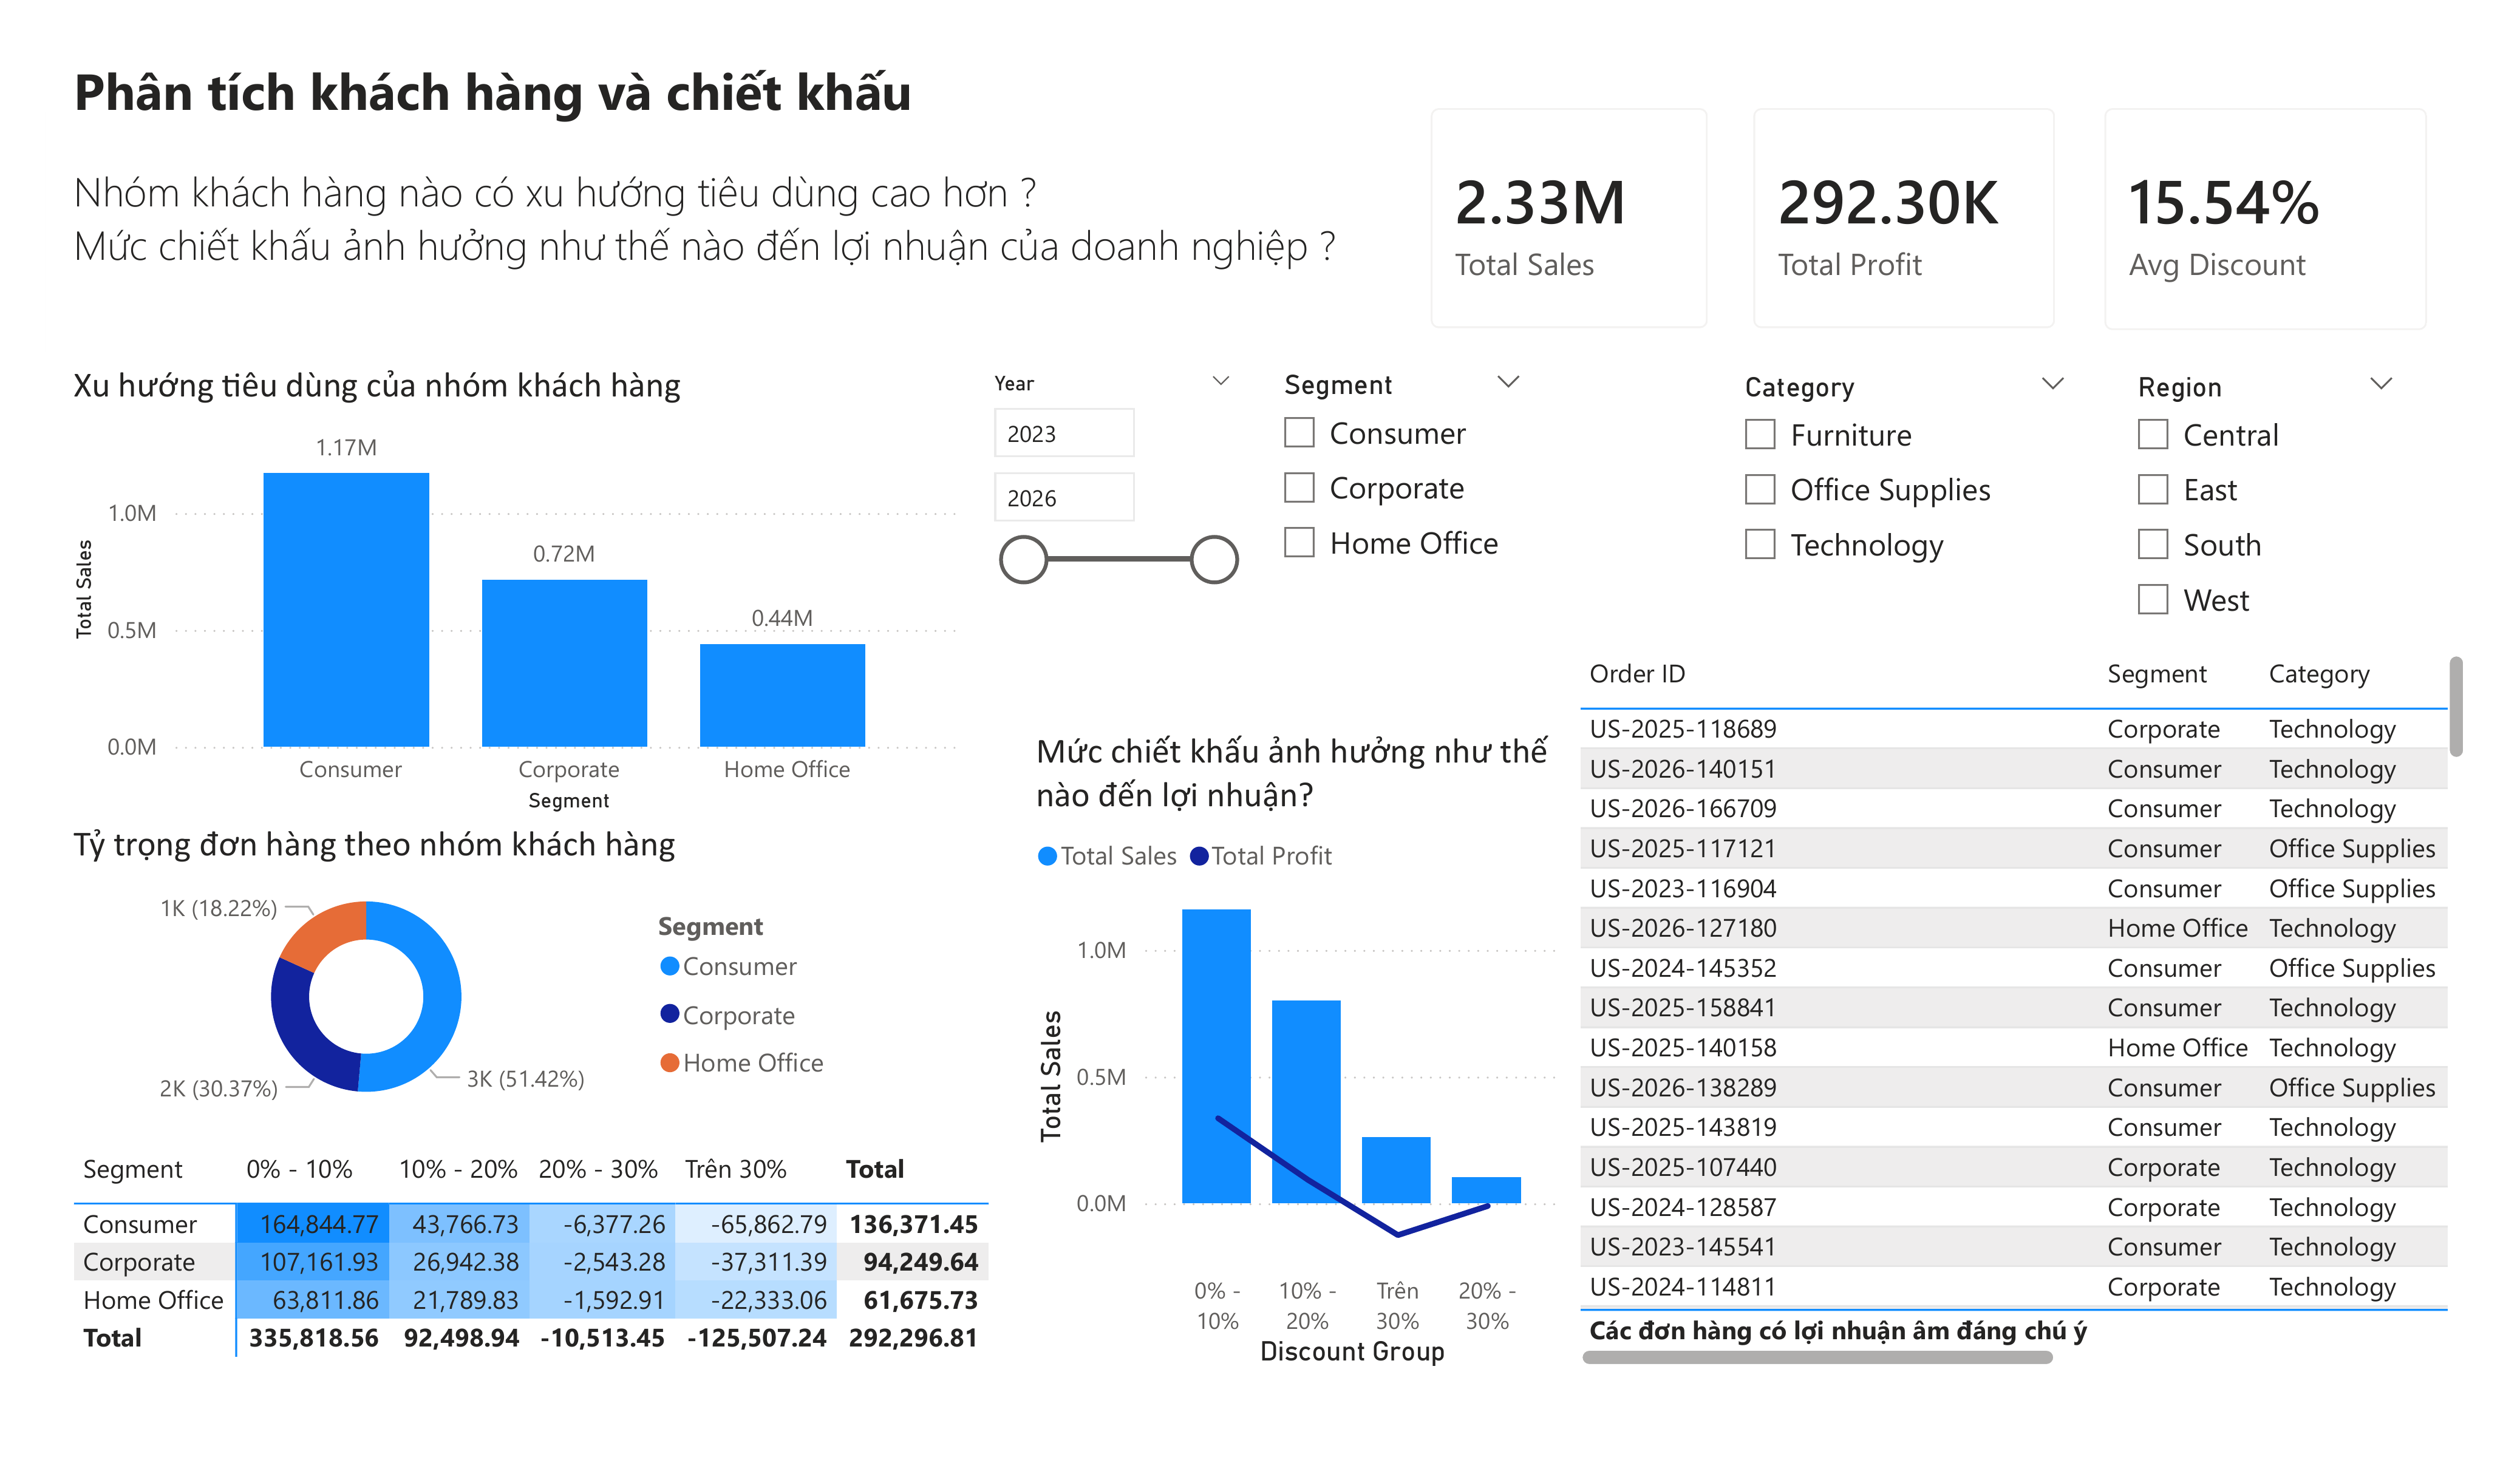
\includegraphics[width=0.95\textwidth]{images/anh_chuong3/dashboard_khach_hang_chiet_khau.png}
\caption{Trang phân tích khách hàng và chiết khấu trên Power BI}
\label{fig:dashboard-khach-hang-chiet-khau}
\end{figure}

\section{Diễn giải ý nghĩa biểu đồ và bộ lọc trên dashboard}

\refstepcounter{subsection}
\subsection*{\thesubsection\quad Nhóm biểu đồ tổng quan kinh doanh}

Nhóm biểu đồ tổng quan kinh doanh được sử dụng để cung cấp cái nhìn nhanh về tình hình hoạt động của doanh nghiệp. Các thẻ chỉ số như tổng doanh thu, tổng lợi nhuận, số lượng bán và số đơn hàng giúp người xem nắm bắt quy mô kinh doanh ở mức tổng quát. Biểu đồ doanh thu theo thời gian hỗ trợ nhận diện xu hướng tăng giảm của doanh số theo năm, quý hoặc tháng. Đây là nhóm biểu đồ trả lời trực tiếp câu hỏi nghiên cứu về sự thay đổi của doanh số bán hàng theo thời gian.

\refstepcounter{subsection}
\subsection*{\thesubsection\quad Nhóm biểu đồ phân tích khu vực và sản phẩm}

Nhóm biểu đồ khu vực và sản phẩm giúp so sánh hiệu quả kinh doanh giữa các vùng thị trường và các nhóm sản phẩm. Biểu đồ doanh thu theo khu vực cho biết khu vực nào đóng góp doanh thu lớn nhất. Biểu đồ lợi nhuận theo khu vực cho phép đánh giá khu vực nào hoạt động hiệu quả hơn về mặt sinh lời. Bên cạnh đó, biểu đồ lợi nhuận theo danh mục và tiểu danh mục sản phẩm giúp nhận diện nhóm sản phẩm có khả năng tạo lợi nhuận cao hoặc đang gây lỗ. Nhóm biểu đồ này hỗ trợ trả lời các câu hỏi nghiên cứu về khu vực và danh mục sản phẩm mang lại doanh thu, lợi nhuận tốt nhất.

\refstepcounter{subsection}
\subsection*{\thesubsection\quad Nhóm biểu đồ phân tích khách hàng và chiết khấu}

Nhóm biểu đồ khách hàng và chiết khấu tập trung vào hai khía cạnh: phân khúc khách hàng và chính sách giảm giá. Biểu đồ doanh thu theo phân khúc khách hàng giúp xác định nhóm khách hàng có mức tiêu dùng cao hơn. Trong khi đó, biểu đồ lợi nhuận theo nhóm chiết khấu cho thấy tác động của mức giảm giá đến hiệu quả kinh doanh. Nếu chiết khấu tăng nhưng lợi nhuận giảm mạnh, doanh nghiệp cần xem xét lại chính sách khuyến mại để tránh tăng doanh thu nhưng làm giảm hiệu quả sinh lời.

\refstepcounter{subsection}
\subsection*{\thesubsection\quad Ý nghĩa các bộ lọc tương tác}

Các bộ lọc trên dashboard giúp người dùng phân tích dữ liệu theo từng lát cắt cụ thể. Bộ lọc theo năm hỗ trợ so sánh kết quả kinh doanh giữa các giai đoạn. Bộ lọc theo khu vực giúp quan sát riêng từng vùng thị trường. Bộ lọc theo danh mục sản phẩm giúp phân tích sâu từng nhóm hàng. Bộ lọc theo phân khúc khách hàng giúp đánh giá hành vi tiêu dùng của từng nhóm đối tượng. Nhờ các bộ lọc này, dashboard không chỉ trình bày dữ liệu ở mức tổng quan mà còn hỗ trợ người dùng khai thác dữ liệu linh hoạt theo nhu cầu phân tích.

\begin{table}[H]
\centering
\caption{Ý nghĩa phân tích của các thành phần trên dashboard}
\label{tab:y-nghia-dashboard}
\begin{tabular}{p{4.5cm} p{8.5cm}}
\hline
\textbf{Thành phần dashboard} & \textbf{Ý nghĩa phân tích} \\
\hline
Thẻ tổng doanh thu & Cho biết quy mô doanh số của toàn bộ dữ liệu hoặc theo điều kiện lọc cụ thể. \\
\hline
Thẻ tổng lợi nhuận & Đánh giá hiệu quả sinh lời tổng thể của hoạt động bán hàng. \\
\hline
Biểu đồ doanh thu theo thời gian & Nhận diện xu hướng tăng giảm doanh số theo năm, quý hoặc tháng. \\
\hline
Biểu đồ doanh thu/lợi nhuận theo khu vực & So sánh mức đóng góp và hiệu quả kinh doanh giữa các khu vực. \\
\hline
Biểu đồ lợi nhuận theo danh mục sản phẩm & Xác định nhóm sản phẩm tạo lợi nhuận tốt hoặc có hiệu quả thấp. \\
\hline
Biểu đồ doanh thu theo phân khúc khách hàng & Nhận diện nhóm khách hàng có xu hướng tiêu dùng cao hơn. \\
\hline
Biểu đồ chiết khấu và lợi nhuận & Đánh giá tác động của chính sách giảm giá đến lợi nhuận. \\
\hline
Bộ lọc tương tác & Hỗ trợ phân tích dữ liệu theo từng năm, khu vực, sản phẩm hoặc phân khúc khách hàng. \\
\hline
\end{tabular}
\end{table}

\section{Đánh giá khả năng hỗ trợ phân tích của dashboard}

\refstepcounter{subsection}
\subsection*{\thesubsection\quad Khả năng hỗ trợ theo dõi và so sánh dữ liệu}

Dashboard giúp tổng hợp nhiều chỉ tiêu kinh doanh quan trọng trong cùng một giao diện, từ đó hỗ trợ người dùng quan sát nhanh tình hình doanh thu, lợi nhuận, sản phẩm, khu vực và khách hàng. So với việc xem dữ liệu dưới dạng bảng, dashboard giúp quá trình nhận diện xu hướng và so sánh giữa các nhóm trở nên trực quan hơn. Người dùng có thể nhanh chóng nhận ra khu vực nào có doanh thu cao, danh mục nào có lợi nhuận tốt, phân khúc khách hàng nào đóng góp nhiều và mức chiết khấu nào có nguy cơ làm giảm lợi nhuận.

\refstepcounter{subsection}
\subsection*{\thesubsection\quad Khả năng hỗ trợ trả lời câu hỏi nghiên cứu}

Dashboard có khả năng hỗ trợ trả lời các câu hỏi nghiên cứu đã đặt ra trong đề tài. Cụ thể, biểu đồ doanh thu theo thời gian giúp đánh giá sự thay đổi của doanh số qua các năm và tháng. Biểu đồ theo khu vực giúp xác định vùng thị trường có đóng góp cao nhất. Biểu đồ theo danh mục và tiểu danh mục sản phẩm giúp nhận diện nhóm hàng mang lại lợi nhuận tốt. Biểu đồ theo phân khúc khách hàng giúp xác định nhóm khách hàng có xu hướng tiêu dùng cao hơn. Cuối cùng, biểu đồ liên quan đến chiết khấu và lợi nhuận giúp đánh giá ảnh hưởng của chính sách giảm giá đến hiệu quả kinh doanh.

\refstepcounter{subsection}
\subsection*{\thesubsection\quad Hạn chế của dashboard và định hướng kết nối với mô hình phân tích}

Mặc dù dashboard có khả năng hỗ trợ tốt cho phân tích mô tả và so sánh trực quan, công cụ này vẫn có một số hạn chế. Dashboard chủ yếu giúp trả lời câu hỏi điều gì đã xảy ra và hỗ trợ nhận diện xu hướng trực quan, nhưng chưa đủ để đánh giá sâu mức độ ảnh hưởng của từng biến hoặc dự báo kết quả trong tương lai. Do đó, để nâng cao chiều sâu phân tích, các chương tiếp theo sẽ xây dựng các mô hình phân tích dữ liệu như hồi quy tuyến tính đa biến, Random Forest Regressor, Gradient Boosting Regressor, XGBoost Regressor và K-Means Clustering. Việc kết hợp dashboard với mô hình phân tích giúp đồ án không chỉ dừng lại ở trực quan hóa dữ liệu mà còn mở rộng sang phân tích quan hệ, dự báo và phân nhóm khách hàng.